% Generated by Sphinx.
\def\sphinxdocclass{report}
\documentclass[letterpaper,10pt,french]{sphinxmanual}
\usepackage[utf8]{inputenc}
\DeclareUnicodeCharacter{00A0}{\nobreakspace}
\usepackage{cmap}
\usepackage[T1]{fontenc}
\usepackage{babel}
\usepackage{times}
\usepackage[Sonny]{fncychap}
\usepackage{longtable}
\usepackage{sphinx}
\usepackage{multirow}


\title{Documentation: dashboard professeur et développement dirigé par les tests}
\date{23 March 2015}
\release{0.1}
\author{Bryan Oberson}
\newcommand{\sphinxlogo}{}
\renewcommand{\releasename}{Version}
\makeindex

\makeatletter
\def\PYG@reset{\let\PYG@it=\relax \let\PYG@bf=\relax%
    \let\PYG@ul=\relax \let\PYG@tc=\relax%
    \let\PYG@bc=\relax \let\PYG@ff=\relax}
\def\PYG@tok#1{\csname PYG@tok@#1\endcsname}
\def\PYG@toks#1+{\ifx\relax#1\empty\else%
    \PYG@tok{#1}\expandafter\PYG@toks\fi}
\def\PYG@do#1{\PYG@bc{\PYG@tc{\PYG@ul{%
    \PYG@it{\PYG@bf{\PYG@ff{#1}}}}}}}
\def\PYG#1#2{\PYG@reset\PYG@toks#1+\relax+\PYG@do{#2}}

\expandafter\def\csname PYG@tok@gd\endcsname{\def\PYG@tc##1{\textcolor[rgb]{0.63,0.00,0.00}{##1}}}
\expandafter\def\csname PYG@tok@gu\endcsname{\let\PYG@bf=\textbf\def\PYG@tc##1{\textcolor[rgb]{0.50,0.00,0.50}{##1}}}
\expandafter\def\csname PYG@tok@gt\endcsname{\def\PYG@tc##1{\textcolor[rgb]{0.00,0.27,0.87}{##1}}}
\expandafter\def\csname PYG@tok@gs\endcsname{\let\PYG@bf=\textbf}
\expandafter\def\csname PYG@tok@gr\endcsname{\def\PYG@tc##1{\textcolor[rgb]{1.00,0.00,0.00}{##1}}}
\expandafter\def\csname PYG@tok@cm\endcsname{\let\PYG@it=\textit\def\PYG@tc##1{\textcolor[rgb]{0.25,0.50,0.56}{##1}}}
\expandafter\def\csname PYG@tok@vg\endcsname{\def\PYG@tc##1{\textcolor[rgb]{0.73,0.38,0.84}{##1}}}
\expandafter\def\csname PYG@tok@m\endcsname{\def\PYG@tc##1{\textcolor[rgb]{0.13,0.50,0.31}{##1}}}
\expandafter\def\csname PYG@tok@mh\endcsname{\def\PYG@tc##1{\textcolor[rgb]{0.13,0.50,0.31}{##1}}}
\expandafter\def\csname PYG@tok@cs\endcsname{\def\PYG@tc##1{\textcolor[rgb]{0.25,0.50,0.56}{##1}}\def\PYG@bc##1{\setlength{\fboxsep}{0pt}\colorbox[rgb]{1.00,0.94,0.94}{\strut ##1}}}
\expandafter\def\csname PYG@tok@ge\endcsname{\let\PYG@it=\textit}
\expandafter\def\csname PYG@tok@vc\endcsname{\def\PYG@tc##1{\textcolor[rgb]{0.73,0.38,0.84}{##1}}}
\expandafter\def\csname PYG@tok@il\endcsname{\def\PYG@tc##1{\textcolor[rgb]{0.13,0.50,0.31}{##1}}}
\expandafter\def\csname PYG@tok@go\endcsname{\def\PYG@tc##1{\textcolor[rgb]{0.20,0.20,0.20}{##1}}}
\expandafter\def\csname PYG@tok@cp\endcsname{\def\PYG@tc##1{\textcolor[rgb]{0.00,0.44,0.13}{##1}}}
\expandafter\def\csname PYG@tok@gi\endcsname{\def\PYG@tc##1{\textcolor[rgb]{0.00,0.63,0.00}{##1}}}
\expandafter\def\csname PYG@tok@gh\endcsname{\let\PYG@bf=\textbf\def\PYG@tc##1{\textcolor[rgb]{0.00,0.00,0.50}{##1}}}
\expandafter\def\csname PYG@tok@ni\endcsname{\let\PYG@bf=\textbf\def\PYG@tc##1{\textcolor[rgb]{0.84,0.33,0.22}{##1}}}
\expandafter\def\csname PYG@tok@nl\endcsname{\let\PYG@bf=\textbf\def\PYG@tc##1{\textcolor[rgb]{0.00,0.13,0.44}{##1}}}
\expandafter\def\csname PYG@tok@nn\endcsname{\let\PYG@bf=\textbf\def\PYG@tc##1{\textcolor[rgb]{0.05,0.52,0.71}{##1}}}
\expandafter\def\csname PYG@tok@no\endcsname{\def\PYG@tc##1{\textcolor[rgb]{0.38,0.68,0.84}{##1}}}
\expandafter\def\csname PYG@tok@na\endcsname{\def\PYG@tc##1{\textcolor[rgb]{0.25,0.44,0.63}{##1}}}
\expandafter\def\csname PYG@tok@nb\endcsname{\def\PYG@tc##1{\textcolor[rgb]{0.00,0.44,0.13}{##1}}}
\expandafter\def\csname PYG@tok@nc\endcsname{\let\PYG@bf=\textbf\def\PYG@tc##1{\textcolor[rgb]{0.05,0.52,0.71}{##1}}}
\expandafter\def\csname PYG@tok@nd\endcsname{\let\PYG@bf=\textbf\def\PYG@tc##1{\textcolor[rgb]{0.33,0.33,0.33}{##1}}}
\expandafter\def\csname PYG@tok@ne\endcsname{\def\PYG@tc##1{\textcolor[rgb]{0.00,0.44,0.13}{##1}}}
\expandafter\def\csname PYG@tok@nf\endcsname{\def\PYG@tc##1{\textcolor[rgb]{0.02,0.16,0.49}{##1}}}
\expandafter\def\csname PYG@tok@si\endcsname{\let\PYG@it=\textit\def\PYG@tc##1{\textcolor[rgb]{0.44,0.63,0.82}{##1}}}
\expandafter\def\csname PYG@tok@s2\endcsname{\def\PYG@tc##1{\textcolor[rgb]{0.25,0.44,0.63}{##1}}}
\expandafter\def\csname PYG@tok@vi\endcsname{\def\PYG@tc##1{\textcolor[rgb]{0.73,0.38,0.84}{##1}}}
\expandafter\def\csname PYG@tok@nt\endcsname{\let\PYG@bf=\textbf\def\PYG@tc##1{\textcolor[rgb]{0.02,0.16,0.45}{##1}}}
\expandafter\def\csname PYG@tok@nv\endcsname{\def\PYG@tc##1{\textcolor[rgb]{0.73,0.38,0.84}{##1}}}
\expandafter\def\csname PYG@tok@s1\endcsname{\def\PYG@tc##1{\textcolor[rgb]{0.25,0.44,0.63}{##1}}}
\expandafter\def\csname PYG@tok@gp\endcsname{\let\PYG@bf=\textbf\def\PYG@tc##1{\textcolor[rgb]{0.78,0.36,0.04}{##1}}}
\expandafter\def\csname PYG@tok@sh\endcsname{\def\PYG@tc##1{\textcolor[rgb]{0.25,0.44,0.63}{##1}}}
\expandafter\def\csname PYG@tok@ow\endcsname{\let\PYG@bf=\textbf\def\PYG@tc##1{\textcolor[rgb]{0.00,0.44,0.13}{##1}}}
\expandafter\def\csname PYG@tok@sx\endcsname{\def\PYG@tc##1{\textcolor[rgb]{0.78,0.36,0.04}{##1}}}
\expandafter\def\csname PYG@tok@bp\endcsname{\def\PYG@tc##1{\textcolor[rgb]{0.00,0.44,0.13}{##1}}}
\expandafter\def\csname PYG@tok@c1\endcsname{\let\PYG@it=\textit\def\PYG@tc##1{\textcolor[rgb]{0.25,0.50,0.56}{##1}}}
\expandafter\def\csname PYG@tok@kc\endcsname{\let\PYG@bf=\textbf\def\PYG@tc##1{\textcolor[rgb]{0.00,0.44,0.13}{##1}}}
\expandafter\def\csname PYG@tok@c\endcsname{\let\PYG@it=\textit\def\PYG@tc##1{\textcolor[rgb]{0.25,0.50,0.56}{##1}}}
\expandafter\def\csname PYG@tok@mf\endcsname{\def\PYG@tc##1{\textcolor[rgb]{0.13,0.50,0.31}{##1}}}
\expandafter\def\csname PYG@tok@err\endcsname{\def\PYG@bc##1{\setlength{\fboxsep}{0pt}\fcolorbox[rgb]{1.00,0.00,0.00}{1,1,1}{\strut ##1}}}
\expandafter\def\csname PYG@tok@kd\endcsname{\let\PYG@bf=\textbf\def\PYG@tc##1{\textcolor[rgb]{0.00,0.44,0.13}{##1}}}
\expandafter\def\csname PYG@tok@ss\endcsname{\def\PYG@tc##1{\textcolor[rgb]{0.32,0.47,0.09}{##1}}}
\expandafter\def\csname PYG@tok@sr\endcsname{\def\PYG@tc##1{\textcolor[rgb]{0.14,0.33,0.53}{##1}}}
\expandafter\def\csname PYG@tok@mo\endcsname{\def\PYG@tc##1{\textcolor[rgb]{0.13,0.50,0.31}{##1}}}
\expandafter\def\csname PYG@tok@mi\endcsname{\def\PYG@tc##1{\textcolor[rgb]{0.13,0.50,0.31}{##1}}}
\expandafter\def\csname PYG@tok@kn\endcsname{\let\PYG@bf=\textbf\def\PYG@tc##1{\textcolor[rgb]{0.00,0.44,0.13}{##1}}}
\expandafter\def\csname PYG@tok@o\endcsname{\def\PYG@tc##1{\textcolor[rgb]{0.40,0.40,0.40}{##1}}}
\expandafter\def\csname PYG@tok@kr\endcsname{\let\PYG@bf=\textbf\def\PYG@tc##1{\textcolor[rgb]{0.00,0.44,0.13}{##1}}}
\expandafter\def\csname PYG@tok@s\endcsname{\def\PYG@tc##1{\textcolor[rgb]{0.25,0.44,0.63}{##1}}}
\expandafter\def\csname PYG@tok@kp\endcsname{\def\PYG@tc##1{\textcolor[rgb]{0.00,0.44,0.13}{##1}}}
\expandafter\def\csname PYG@tok@w\endcsname{\def\PYG@tc##1{\textcolor[rgb]{0.73,0.73,0.73}{##1}}}
\expandafter\def\csname PYG@tok@kt\endcsname{\def\PYG@tc##1{\textcolor[rgb]{0.56,0.13,0.00}{##1}}}
\expandafter\def\csname PYG@tok@sc\endcsname{\def\PYG@tc##1{\textcolor[rgb]{0.25,0.44,0.63}{##1}}}
\expandafter\def\csname PYG@tok@sb\endcsname{\def\PYG@tc##1{\textcolor[rgb]{0.25,0.44,0.63}{##1}}}
\expandafter\def\csname PYG@tok@k\endcsname{\let\PYG@bf=\textbf\def\PYG@tc##1{\textcolor[rgb]{0.00,0.44,0.13}{##1}}}
\expandafter\def\csname PYG@tok@se\endcsname{\let\PYG@bf=\textbf\def\PYG@tc##1{\textcolor[rgb]{0.25,0.44,0.63}{##1}}}
\expandafter\def\csname PYG@tok@sd\endcsname{\let\PYG@it=\textit\def\PYG@tc##1{\textcolor[rgb]{0.25,0.44,0.63}{##1}}}

\def\PYGZbs{\char`\\}
\def\PYGZus{\char`\_}
\def\PYGZob{\char`\{}
\def\PYGZcb{\char`\}}
\def\PYGZca{\char`\^}
\def\PYGZam{\char`\&}
\def\PYGZlt{\char`\<}
\def\PYGZgt{\char`\>}
\def\PYGZsh{\char`\#}
\def\PYGZpc{\char`\%}
\def\PYGZdl{\char`\$}
\def\PYGZhy{\char`\-}
\def\PYGZsq{\char`\'}
\def\PYGZdq{\char`\"}
\def\PYGZti{\char`\~}
% for compatibility with earlier versions
\def\PYGZat{@}
\def\PYGZlb{[}
\def\PYGZrb{]}
\makeatother

\renewcommand\PYGZsq{\textquotesingle}

\begin{document}

\maketitle
\tableofcontents
\phantomsection\label{index::doc}



\chapter{Fonctionnalités du dashboard}
\label{dashboard:fonctionnalites-du-dashboard}\label{dashboard::doc}\label{dashboard:conception-du-dashboard-professeur-et-developpement-dirige-par-les-tests}

\section{Ajouter un groupe}
\label{dashboard:ajouter-un-groupe}
La fonctionnalité de base de ce dashboard est la création de groupe. En créant
un groupe, le professeur sera par la suite capable de le gérer en gérant les
membres qui s'y trouvent mais aussi en y assignant des devoirs.

Pour créer un groupe, il suffit de se rendre sur Nouveau groupe, tout en bas
dans le menu de gauche. Cette action fera apparaître le formulaire de création
de groupe.
\begin{figure}[htbp]
\centering
\capstart

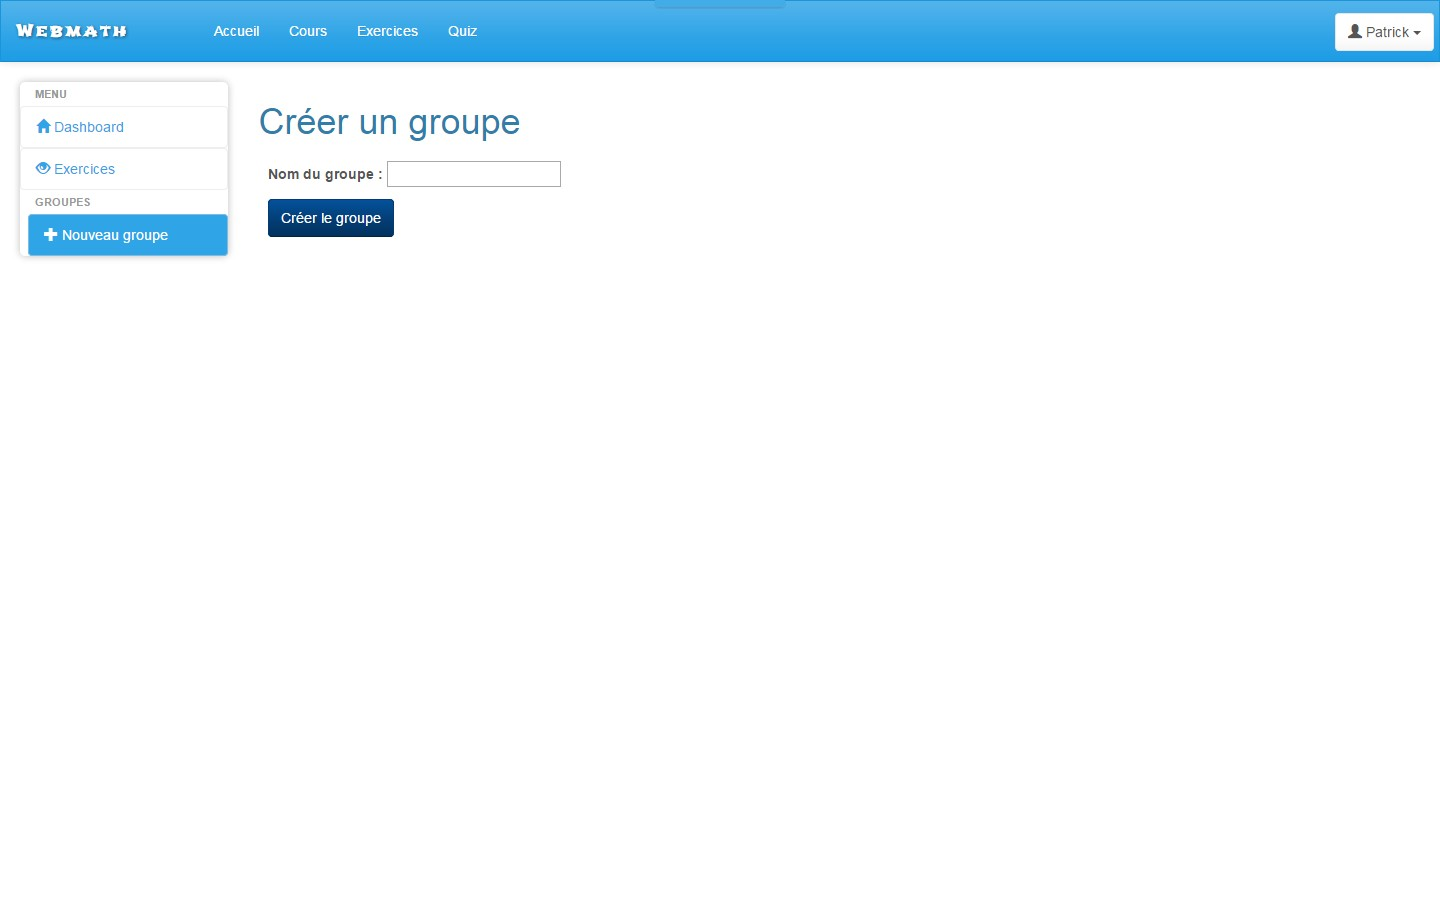
\includegraphics[width=0.600\linewidth]{Newclass.jpg}
\caption{Formulaire de création de groupe}\end{figure}

La seule exigence présente lors de la création d'un groupe est le nom. Une fois
le groupe créé, l'utilisateur actuel est automatiquement défini en tant que
professeur pour le groupe.

Le groupe précédemment créé sera désormais affiché en permanence dans le menu
de gauche du professeur, ce qui lui permet d'accéder à ses informations.


\section{Gérer un groupe}
\label{dashboard:gerer-un-groupe}

\subsection{Gérer les membres du groupe}
\label{dashboard:gerer-les-membres-du-groupe}
Depuis cette page, le professeur peut gérer les membres qui sont actuellement
enregistrés dans le groupe.

Il peut tout d'abord rajouter les élèves ou professeurs qu'il souhaite en
entrant leur nom d'utilisateur dans le champ à disposition.
\begin{figure}[htbp]
\centering
\capstart

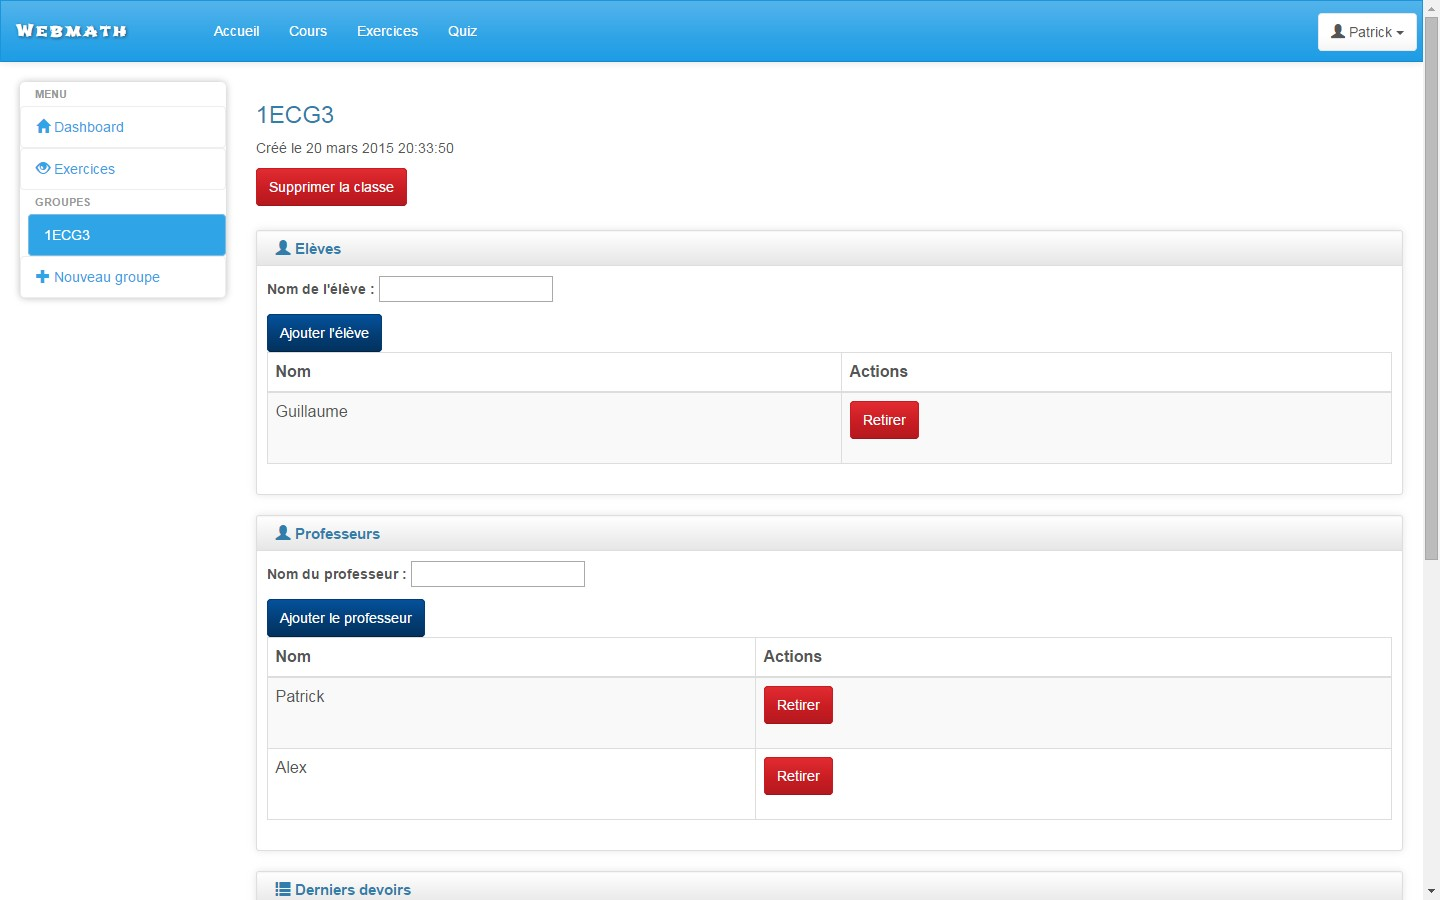
\includegraphics[width=0.600\linewidth]{class.jpg}
\caption{Page d'administration d'un groupe}\end{figure}

Si le nom d'utilisateur rentré correspond bien à un étudiant ou à un professeur,
cet utilisateur sera rajouté dans la liste des membres.
\begin{figure}[htbp]
\centering
\capstart

\includegraphics[width=0.600\linewidth]{classAjouterMembres.jpg}
\caption{Ce à quoi ressemble la page une fois que des membres ont été rajoutés}\end{figure}

Au contraire, si aucun utilisateur n'a été trouvé ou si l'utilisateur ne
correspond pas au rôle qu'il lui est donné (par exemple si c'est un
professeur et qu'il a été ajouté aux étudiants), le site renvoiera un message
d'erreur.
\begin{figure}[htbp]
\centering
\capstart

\includegraphics[width=0.600\linewidth]{classAjouterMembresEchec.jpg}
\caption{Message d'erreur retourné si l'utilisateur n'est pas valable}\end{figure}

Une fois ajouté, un membre peut facilement être retiré du groupe grâce au bouton
Retirer qui se trouve à côté de son nom.


\subsection{Gérer un devoir}
\label{dashboard:gerer-un-devoir}
Un professeur peut bien évidemment donner des devoirs à son groupe.

Un devoir peut-être un exercice, un quiz ou un cours, tous les trois
pouvant avoir été créé par un autre utilisateur.

Pour assigner un devoir, il suffit de savoir l'id de l'exercice, quiz ou cours,
et de préciser grâce au menu à choix de quel type de devoir il s'agit.
\begin{figure}[htbp]
\centering
\capstart

\includegraphics[width=0.600\linewidth]{classDevoir.jpg}
\caption{Différents champs à compléter pour assigner un devoir}\end{figure}

Comme pour les fonctionnalités précédentes, si aucun exercice, quiz ou cours
n'a pu être associé à l'id entrée, un message d'erreur sera renvoyé.

Un devoir peut être à tout moment retiré grâce au bouton Retirer à sa droite.


\section{Voir ses exercices}
\label{dashboard:voir-ses-exercices}
Dans le menu de gauche, il y a un bouton nommé Exercices. C'est depuis cette
page que le professeur pourra voir ses exercices, ses quiz et ses cours.
\begin{figure}[htbp]
\centering
\capstart

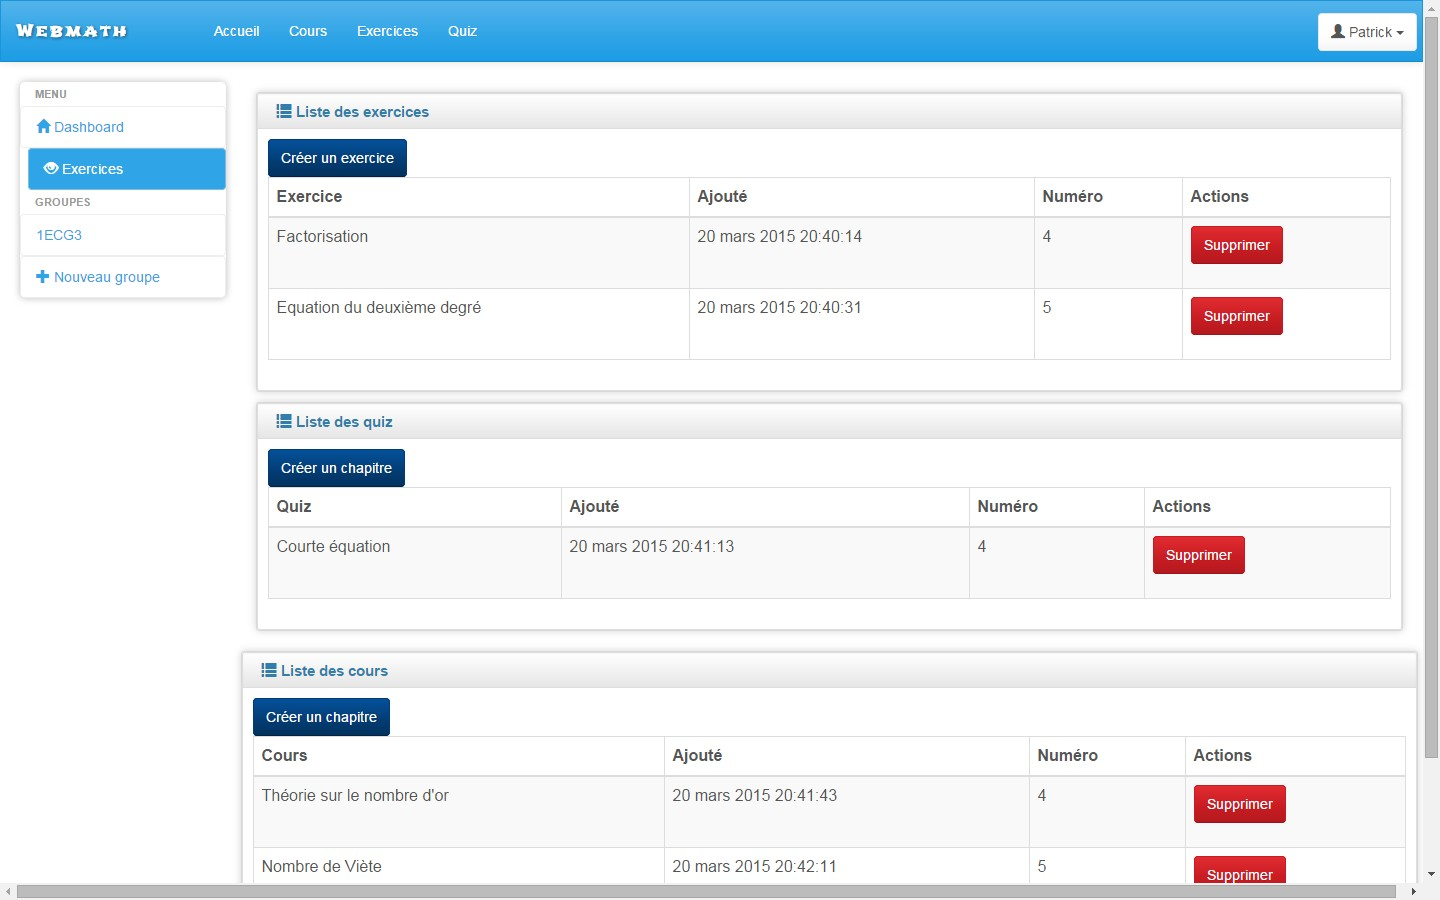
\includegraphics[width=0.600\linewidth]{exercices.jpg}
\caption{Ce à quoi ressemble la page Exercices}\end{figure}

Pour chaque activité que le professeur aura créé, il pourra voir le titre qu'il
lui a donné, la date à laquelle il l'a créé et l'id qui lui sera utile s'il veut
l'assigner en tant que devoir à un de ses groupes.

Il peut bien évidemment supprimer une activité en utilisant le bouton Supprimer
se trouvant dans la dernière colonne du tableau.

Si le professeur souhaite créer une nouvelle activité, il n'a qu'à utiliser le
bouton Créer en haut du tableau qui le redirigera directement au formulaire de
création.


\section{Changer de mot de passe}
\label{dashboard:changer-de-mot-de-passe}
Peu importe sur quelle page il se trouve, le professeur peut accéder à un menu
déroulant en haut à droite de cette page.
\begin{figure}[htbp]
\centering
\capstart

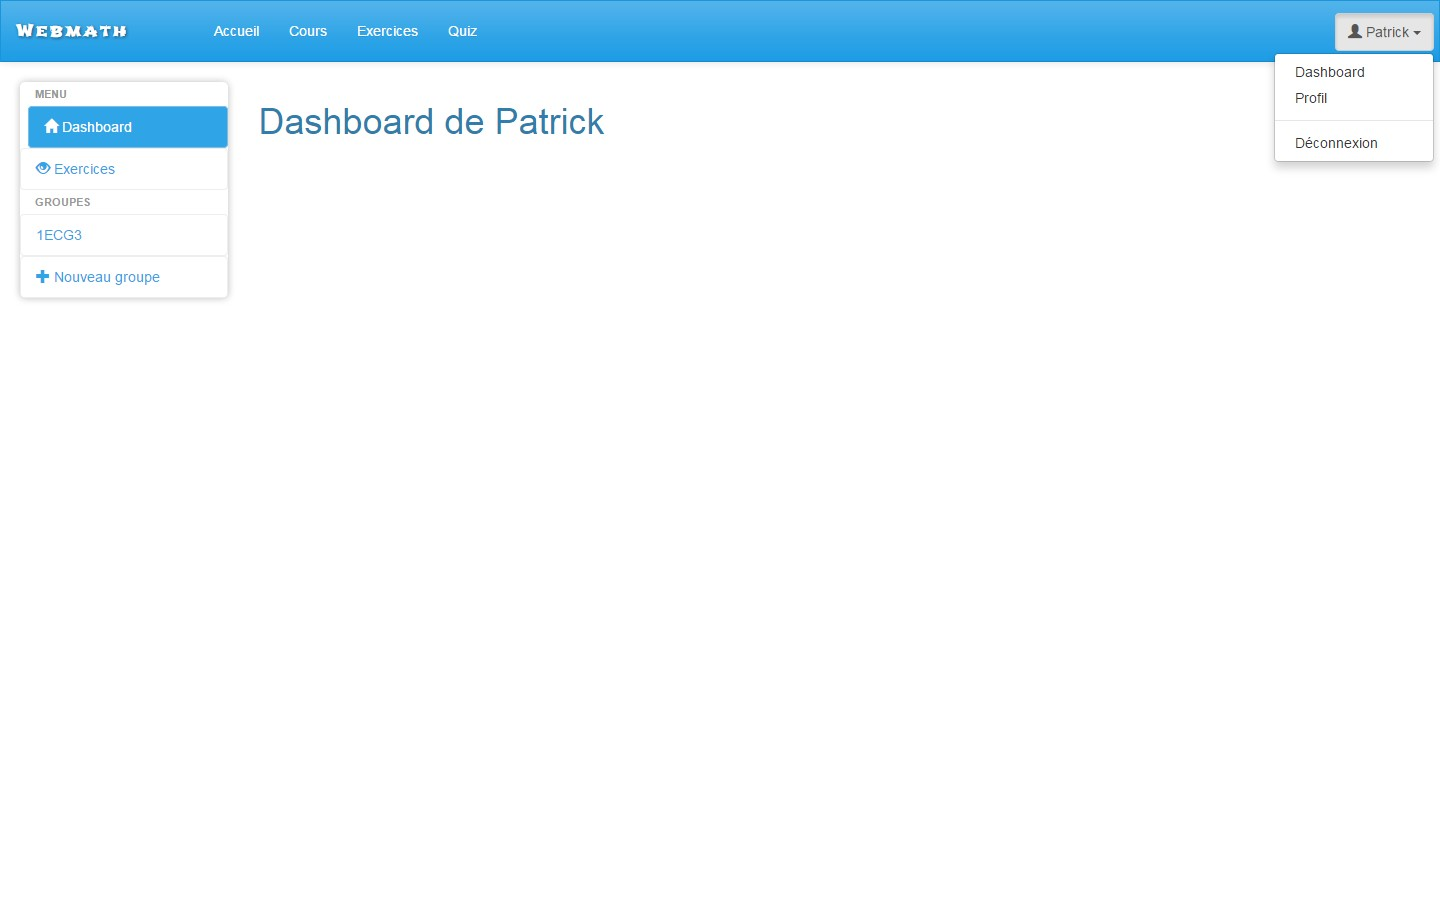
\includegraphics[width=0.600\linewidth]{menuDeroulant.jpg}
\caption{Apparence du menu déroulant}\end{figure}

Dashboard amène le professeur sur l'accueil de son dashboard, Déconnexion le
déconnecte et Profil l'amène sur un formulaire de changement de mot de passe.

Pour le modifier, le professeur n'a qu'à remplir les deux champs et à valider.
Si tout a été rentré correctement, le mot de passe sera correctement modifié.
\begin{figure}[htbp]
\centering
\capstart

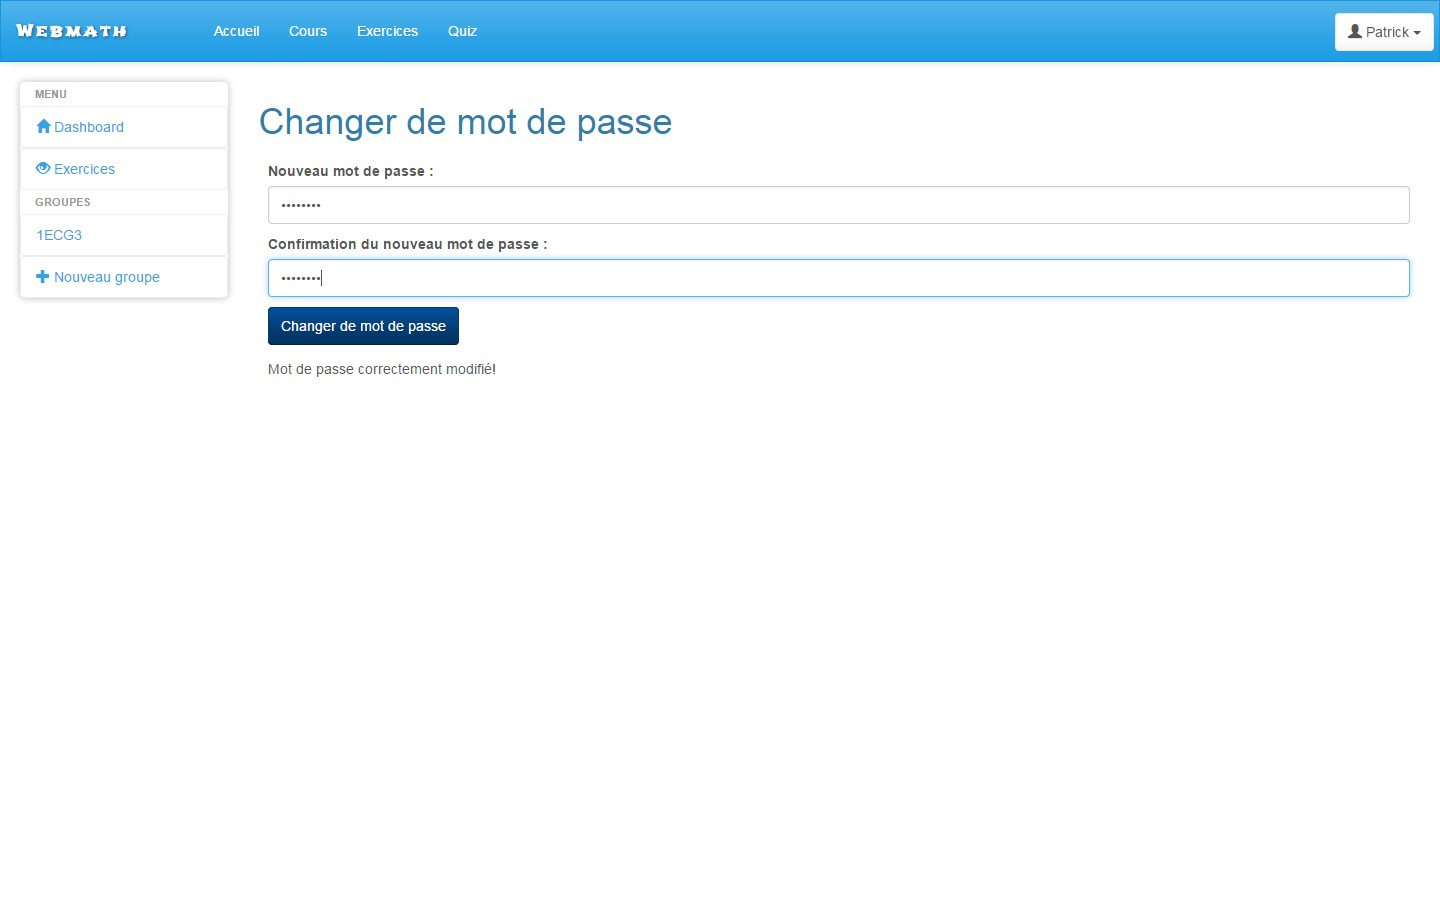
\includegraphics[width=0.600\linewidth]{passwordSuccess.jpg}
\caption{Message pour confirmer que le changement de mot de passe a correctement eu
lieu}\end{figure}

Au contraire, s'il y a une erreur, un message d'erreur sera retourné.
\begin{figure}[htbp]
\centering
\capstart

\includegraphics[width=0.600\linewidth]{passwordFail.jpg}
\caption{Message d'erreur retourné si les champs n'ont pas correctement été remplis}\end{figure}


\chapter{Guide du développeur}
\label{documentation:guide-du-developpeur}\label{documentation::doc}

\section{Utilité des différents fichiers de mon projet}
\label{documentation:utilite-des-differents-fichiers-de-mon-projet}

\subsection{Dossier \texttt{static}}
\label{documentation:dossier-static}
Le dossier static est utilisé pour garder tous les fichiers tel que les images,
les fichiers CSS ou les fichiers Javascript.
Dans cette application, il contient les dossiers suivants:
\begin{itemize}
\item {} 
\code{bower\_components}: ce dossier contient tous les éléments du front-end
qui possèdent des dépendances, comme les fichiers \code{bootstrap} ou des
fichiers de base pour \code{jquery}.

\item {} 
\code{css}: dans ce dossier se trouvent tous les fichiers css qui sont
nécessaires pour le design du site.

\item {} 
\code{fonts}: le dossier \code{fonts} de l'application dashboard contient toutes
les informations relatives aux petits signes (\code{glyphicons}) qui sont
utilisés dans le dashboard, comme le + devant «Nouveau groupe».

\end{itemize}


\subsection{Dossier \texttt{templates}}
\label{documentation:dossier-templates}
Dans le dossier \code{templates} se trouvent tous les fichiers \code{html} qui sont
utilisés dans l'application et retournés par les différentes vues.


\subsection{Fichiers propres à l'application}
\label{documentation:fichiers-propres-a-l-application}
Les applications Django possèdent les fichiers de base suivants:
\begin{itemize}
\item {} 
\code{models.py} qui est utilisé pour créer les différents modèles et leur
attribuer des champs

\item {} 
\code{admin.py} est utilisé pour signaler à Django quels sont les modèles qui
doivent apparaître dans l'application admin. Une fois qu'ils y apparaissent,
il est possible de créer, modifier ou supprimer n'importe quel object depuis
cette application.application

\item {} 
Le fichier \code{forms.py} est celui dans lequel on peut entrer les différents
formulaires dont l'on a besoin pour l'application.

\item {} 
C'est dans \code{views.py} que l'on peut stocker des variables nécessaires
dans certains templates, mais aussi réaliser certaines actions comme la
suppression d'un objet. A la fin d'une vue, on retourne souvent un fichiers
\code{html} ou on redirige vers une autre vue.

\item {} 
Le fichier \code{urls.py} contient les informations concernant les différentes
urls accessibles par l'utilisateur et quelles vues sont censées être
utilisées.

\end{itemize}


\subsection{Fichiers uniques de Django}
\label{documentation:fichiers-uniques-de-django}
On peut modifier le fichier \code{settings.py} afin de définir la zone temporelle
dans laquelle on se trouve, mais aussi les applications qu'un projet doit
gérer ou encore l'emplacement du fichier \code{static}. Il sert donc de
configuration de base pour un projet.

Il y a aussi un autre fichiers \code{urls.py} qui, lui, est très utile si l'on doit
s'occuper de plusieurs applications à la fois. En effet, on peut définir le
début de l'url et rediriger vers un autre fichier \code{urls.py}.


\section{Modèles}
\label{documentation:modeles}

\subsection{Modèles utilisés pour le dashboard}
\label{documentation:modeles-utilises-pour-le-dashboard}
\begin{Verbatim}[commandchars=\\\{\},numbers=left,firstnumber=1,stepnumber=1]
\PYG{k+kn}{from} \PYG{n+nn}{django.db} \PYG{k+kn}{import} \PYG{n}{models}
\PYG{k+kn}{from} \PYG{n+nn}{django.contrib.auth.models} \PYG{k+kn}{import} \PYG{n}{User}


\PYG{c}{\PYGZsh{}Profile de base découlant de User}

\PYG{k}{class} \PYG{n+nc}{BaseProfile}\PYG{p}{(}\PYG{n}{models}\PYG{o}{.}\PYG{n}{Model}\PYG{p}{)}\PYG{p}{:}
    \PYG{n}{user} \PYG{o}{=} \PYG{n}{models}\PYG{o}{.}\PYG{n}{OneToOneField}\PYG{p}{(}\PYG{n}{User}\PYG{p}{)} \PYG{c}{\PYGZsh{}Donne les attributs de User à BaseProfile}
    \PYG{n}{avatar} \PYG{o}{=} \PYG{n}{models}\PYG{o}{.}\PYG{n}{ImageField}\PYG{p}{(}\PYG{n}{null}\PYG{o}{=}\PYG{n+nb+bp}{True}\PYG{p}{,} \PYG{n}{blank}\PYG{o}{=}\PYG{n+nb+bp}{True}\PYG{p}{,} \PYG{n}{upload\PYGZus{}to}\PYG{o}{=}\PYG{l+s}{\PYGZdq{}}\PYG{l+s}{avatars/}\PYG{l+s}{\PYGZdq{}}\PYG{p}{)}
        
    \PYG{k}{class} \PYG{n+nc}{Meta}\PYG{p}{:}
        \PYG{n}{abstract} \PYG{o}{=} \PYG{n+nb+bp}{True}


\PYG{c}{\PYGZsh{}Les deux modèles héritent de BaseProfile et donc de User}

\PYG{k}{class} \PYG{n+nc}{Teacher}\PYG{p}{(}\PYG{n}{BaseProfile}\PYG{p}{)}\PYG{p}{:}

    \PYG{k}{def} \PYG{n+nf}{\PYGZus{}\PYGZus{}str\PYGZus{}\PYGZus{}}\PYG{p}{(}\PYG{n+nb+bp}{self}\PYG{p}{)}\PYG{p}{:}
        \PYG{k}{return} \PYG{l+s}{\PYGZdq{}}\PYG{l+s}{Professeur \PYGZob{}0\PYGZcb{}}\PYG{l+s}{\PYGZdq{}}\PYG{o}{.}\PYG{n}{format}\PYG{p}{(}\PYG{n+nb+bp}{self}\PYG{o}{.}\PYG{n}{user}\PYG{o}{.}\PYG{n}{username}\PYG{p}{)}

\PYG{k}{class} \PYG{n+nc}{Student}\PYG{p}{(}\PYG{n}{BaseProfile}\PYG{p}{)}\PYG{p}{:}

    \PYG{k}{def} \PYG{n+nf}{\PYGZus{}\PYGZus{}str\PYGZus{}\PYGZus{}}\PYG{p}{(}\PYG{n+nb+bp}{self}\PYG{p}{)}\PYG{p}{:}
        \PYG{k}{return} \PYG{l+s}{\PYGZdq{}}\PYG{l+s}{Etudiant \PYGZob{}0\PYGZcb{}}\PYG{l+s}{\PYGZdq{}}\PYG{o}{.}\PYG{n}{format}\PYG{p}{(}\PYG{n+nb+bp}{self}\PYG{o}{.}\PYG{n}{user}\PYG{o}{.}\PYG{n}{username}\PYG{p}{)}
        

\PYG{c}{\PYGZsh{}}
\PYG{c}{\PYGZsh{} Modèle de Keran pour les cours}
\PYG{c}{\PYGZsh{}}

\PYG{k}{class} \PYG{n+nc}{Course}\PYG{p}{(}\PYG{n}{models}\PYG{o}{.}\PYG{n}{Model}\PYG{p}{)}\PYG{p}{:}
    \PYG{n}{title} \PYG{o}{=} \PYG{n}{models}\PYG{o}{.}\PYG{n}{CharField}\PYG{p}{(}\PYG{n}{max\PYGZus{}length}\PYG{o}{=}\PYG{l+m+mi}{30}\PYG{p}{,} \PYG{n}{unique}\PYG{o}{=}\PYG{n+nb+bp}{True}\PYG{p}{)}
    \PYG{n}{description} \PYG{o}{=} \PYG{n}{models}\PYG{o}{.}\PYG{n}{TextField}\PYG{p}{(}\PYG{p}{)}
    \PYG{n}{difficulty} \PYG{o}{=} \PYG{n}{models}\PYG{o}{.}\PYG{n}{IntegerField}\PYG{p}{(}\PYG{p}{)}
    \PYG{n}{published} \PYG{o}{=} \PYG{n}{models}\PYG{o}{.}\PYG{n}{BooleanField}\PYG{p}{(}\PYG{n}{default}\PYG{o}{=}\PYG{n+nb+bp}{False}\PYG{p}{)}
    
    \PYG{n}{author} \PYG{o}{=} \PYG{n}{models}\PYG{o}{.}\PYG{n}{ForeignKey}\PYG{p}{(}\PYG{n}{Teacher}\PYG{p}{)}
    \PYG{c}{\PYGZsh{}chapter = models.ForeignKey(\PYGZsq{}teachers.Chapter\PYGZsq{}, related\PYGZus{}name=\PYGZdq{}courses\PYGZdq{})}
    \PYG{n}{favorites} \PYG{o}{=} \PYG{n}{models}\PYG{o}{.}\PYG{n}{ManyToManyField}\PYG{p}{(}\PYG{n}{User}\PYG{p}{,} \PYG{n}{related\PYGZus{}name}\PYG{o}{=}\PYG{l+s}{\PYGZdq{}}\PYG{l+s}{favorite\PYGZus{}courses}\PYG{l+s}{\PYGZdq{}}\PYG{p}{,} \PYG{n}{blank}\PYG{o}{=}\PYG{n+nb+bp}{True}\PYG{p}{,} \PYG{n}{null}\PYG{o}{=}\PYG{n+nb+bp}{True}\PYG{p}{)}
    \PYG{c}{\PYGZsh{} videos = models.ManyToManyField(Video)}
    \PYG{c}{\PYGZsh{} images = models.ManyToManyField(Image)}
    \PYG{c}{\PYGZsh{} definitions = models.ManyToManyField(Definition)}
    
    \PYG{n}{created\PYGZus{}at} \PYG{o}{=} \PYG{n}{models}\PYG{o}{.}\PYG{n}{DateTimeField}\PYG{p}{(}\PYG{n}{auto\PYGZus{}now\PYGZus{}add}\PYG{o}{=}\PYG{n+nb+bp}{True}\PYG{p}{)}
    \PYG{n}{updated\PYGZus{}at} \PYG{o}{=} \PYG{n}{models}\PYG{o}{.}\PYG{n}{DateTimeField}\PYG{p}{(}\PYG{n}{auto\PYGZus{}now}\PYG{o}{=}\PYG{n+nb+bp}{True}\PYG{p}{)}

    \PYG{k}{def} \PYG{n+nf}{\PYGZus{}\PYGZus{}str\PYGZus{}\PYGZus{}}\PYG{p}{(}\PYG{n+nb+bp}{self}\PYG{p}{)}\PYG{p}{:}
      \PYG{k}{return} \PYG{n+nb+bp}{self}\PYG{o}{.}\PYG{n}{title}
      
\PYG{c}{\PYGZsh{}}
\PYG{c}{\PYGZsh{} Modèle de Florian pour les exercices}
\PYG{c}{\PYGZsh{}}

\PYG{k}{class} \PYG{n+nc}{Exercise}\PYG{p}{(}\PYG{n}{models}\PYG{o}{.}\PYG{n}{Model}\PYG{p}{)}\PYG{p}{:}
    
    \PYG{n}{owner} \PYG{o}{=} \PYG{n}{models}\PYG{o}{.}\PYG{n}{ForeignKey}\PYG{p}{(}\PYG{n}{Teacher}\PYG{p}{)}  \PYG{c}{\PYGZsh{} créateur de l\PYGZsq{}exercice   }
    \PYG{n}{created\PYGZus{}on} \PYG{o}{=} \PYG{n}{models}\PYG{o}{.}\PYG{n}{DateTimeField}\PYG{p}{(}\PYG{n}{auto\PYGZus{}now\PYGZus{}add}\PYG{o}{=}\PYG{n+nb+bp}{True}\PYG{p}{)} \PYG{c}{\PYGZsh{} Date de création}
    \PYG{n}{updated\PYGZus{}on} \PYG{o}{=} \PYG{n}{models}\PYG{o}{.}\PYG{n}{DateTimeField}\PYG{p}{(}\PYG{n}{auto\PYGZus{}now}\PYG{o}{=}\PYG{n+nb+bp}{True}\PYG{p}{)}
    \PYG{n}{title} \PYG{o}{=} \PYG{n}{models}\PYG{o}{.}\PYG{n}{CharField}\PYG{p}{(}\PYG{n}{max\PYGZus{}length}\PYG{o}{=}\PYG{l+m+mi}{30}\PYG{p}{)} \PYG{c}{\PYGZsh{} C\PYGZsq{}est le titre de l\PYGZsq{}exercice ( factorisation ou développement)}
    \PYG{n}{equation} \PYG{o}{=} \PYG{n}{models}\PYG{o}{.}\PYG{n}{CharField}\PYG{p}{(}\PYG{n}{max\PYGZus{}length}\PYG{o}{=}\PYG{l+m+mi}{50}\PYG{p}{)} \PYG{c}{\PYGZsh{} C\PYGZsq{}est l\PYGZsq{}équation entrée par le professeur}
    \PYG{n}{grade} \PYG{o}{=} \PYG{n}{models}\PYG{o}{.}\PYG{n}{CharField}\PYG{p}{(}\PYG{n}{max\PYGZus{}length}\PYG{o}{=}\PYG{l+m+mi}{60}\PYG{p}{)} \PYG{c}{\PYGZsh{} donnée une note de difficulté à l\PYGZsq{}exercice}
    \PYG{n}{correction} \PYG{o}{=} \PYG{n}{models}\PYG{o}{.}\PYG{n}{CharField}\PYG{p}{(}\PYG{n}{max\PYGZus{}length} \PYG{o}{=} \PYG{l+m+mi}{200}\PYG{p}{)} \PYG{c}{\PYGZsh{} Ceci est le corrigé de l\PYGZsq{}exercice ( obligatoire )}
    \PYG{k}{def} \PYG{n+nf}{\PYGZus{}\PYGZus{}str\PYGZus{}\PYGZus{}}\PYG{p}{(}\PYG{n+nb+bp}{self}\PYG{p}{)}\PYG{p}{:}
        \PYG{k}{return} \PYG{n+nb+bp}{self}\PYG{o}{.}\PYG{n}{title}
        
\PYG{c}{\PYGZsh{}}
\PYG{c}{\PYGZsh{} Modèle de Benoit pour les quiz}
\PYG{c}{\PYGZsh{}}

\PYG{k}{class} \PYG{n+nc}{Quiz}\PYG{p}{(}\PYG{n}{models}\PYG{o}{.}\PYG{n}{Model}\PYG{p}{)}\PYG{p}{:} \PYG{c}{\PYGZsh{}Infos générales sur le quiz}
    \PYG{n}{title} \PYG{o}{=} \PYG{n}{models}\PYG{o}{.}\PYG{n}{CharField}\PYG{p}{(}\PYG{n}{max\PYGZus{}length}\PYG{o}{=}\PYG{l+m+mi}{100}\PYG{p}{)}
    \PYG{n}{creation\PYGZus{}date} \PYG{o}{=} \PYG{n}{models}\PYG{o}{.}\PYG{n}{DateTimeField}\PYG{p}{(}\PYG{n}{auto\PYGZus{}now\PYGZus{}add}\PYG{o}{=}\PYG{n+nb+bp}{True}\PYG{p}{)}
    \PYG{n}{code} \PYG{o}{=} \PYG{n}{models}\PYG{o}{.}\PYG{n}{CharField}\PYG{p}{(}\PYG{n}{max\PYGZus{}length}\PYG{o}{=}\PYG{l+m+mi}{1000}\PYG{p}{)} \PYG{c}{\PYGZsh{}Format texte du quiz}
    \PYG{n}{author} \PYG{o}{=} \PYG{n}{models}\PYG{o}{.}\PYG{n}{ForeignKey}\PYG{p}{(}\PYG{n}{Teacher}\PYG{p}{)}
    \PYG{c}{\PYGZsh{}id\PYGZus{}chapter = models.ForeignKey(\PYGZsq{}teachers.Chapter\PYGZsq{})}
    
    \PYG{k}{def} \PYG{n+nf}{\PYGZus{}\PYGZus{}str\PYGZus{}\PYGZus{}}\PYG{p}{(}\PYG{n+nb+bp}{self}\PYG{p}{)}\PYG{p}{:}
        \PYG{k}{return} \PYG{n+nb+bp}{self}\PYG{o}{.}\PYG{n}{title}
        
        
        

\PYG{c}{\PYGZsh{}Modèle pour les groupes}
\PYG{k}{class} \PYG{n+nc}{Group}\PYG{p}{(}\PYG{n}{models}\PYG{o}{.}\PYG{n}{Model}\PYG{p}{)}\PYG{p}{:}
    \PYG{n}{name} \PYG{o}{=} \PYG{n}{models}\PYG{o}{.}\PYG{n}{CharField}\PYG{p}{(}\PYG{n}{max\PYGZus{}length}\PYG{o}{=}\PYG{l+m+mi}{30}\PYG{p}{)}
    \PYG{n}{teacher} \PYG{o}{=} \PYG{n}{models}\PYG{o}{.}\PYG{n}{ManyToManyField}\PYG{p}{(}\PYG{n}{Teacher}\PYG{p}{,} \PYG{n}{through}\PYG{o}{=}\PYG{l+s}{\PYGZsq{}}\PYG{l+s}{GroupMembers}\PYG{l+s}{\PYGZsq{}}\PYG{p}{)}
    \PYG{n}{student} \PYG{o}{=} \PYG{n}{models}\PYG{o}{.}\PYG{n}{ManyToManyField}\PYG{p}{(}\PYG{n}{Student}\PYG{p}{,} \PYG{n}{through} \PYG{o}{=} \PYG{l+s}{\PYGZsq{}}\PYG{l+s}{GroupMembers}\PYG{l+s}{\PYGZsq{}}\PYG{p}{)}
    \PYG{n}{homeworkExercise} \PYG{o}{=} \PYG{n}{models}\PYG{o}{.}\PYG{n}{ManyToManyField}\PYG{p}{(}\PYG{n}{Exercise}\PYG{p}{,} \PYG{n}{through} \PYG{o}{=} \PYG{l+s}{\PYGZsq{}}\PYG{l+s}{AssignHomework}\PYG{l+s}{\PYGZsq{}}\PYG{p}{)} \PYG{c}{\PYGZsh{}uniquement les devoirs exercices}
    \PYG{n}{homeworkCourse} \PYG{o}{=} \PYG{n}{models}\PYG{o}{.}\PYG{n}{ManyToManyField}\PYG{p}{(}\PYG{n}{Course}\PYG{p}{,} \PYG{n}{through} \PYG{o}{=} \PYG{l+s}{\PYGZsq{}}\PYG{l+s}{AssignHomework}\PYG{l+s}{\PYGZsq{}}\PYG{p}{)} \PYG{c}{\PYGZsh{}uniquement les devoirs quiz}
    \PYG{n}{homeworkQuiz} \PYG{o}{=} \PYG{n}{models}\PYG{o}{.}\PYG{n}{ManyToManyField}\PYG{p}{(}\PYG{n}{Quiz}\PYG{p}{,} \PYG{n}{through} \PYG{o}{=} \PYG{l+s}{\PYGZsq{}}\PYG{l+s}{AssignHomework}\PYG{l+s}{\PYGZsq{}}\PYG{p}{)} \PYG{c}{\PYGZsh{}uniquement les devoirs cours}
    \PYG{n}{created\PYGZus{}on} \PYG{o}{=} \PYG{n}{models}\PYG{o}{.}\PYG{n}{DateTimeField}\PYG{p}{(}\PYG{n}{auto\PYGZus{}now}\PYG{o}{=}\PYG{n+nb+bp}{True}\PYG{p}{)}
    
    \PYG{k}{def} \PYG{n+nf}{\PYGZus{}\PYGZus{}str\PYGZus{}\PYGZus{}}\PYG{p}{(}\PYG{n+nb+bp}{self}\PYG{p}{)}\PYG{p}{:}
        \PYG{k}{return}\PYG{l+s}{\PYGZdq{}}\PYG{l+s}{Classe \PYGZob{}0\PYGZcb{}}\PYG{l+s}{\PYGZdq{}}\PYG{o}{.}\PYG{n}{format}\PYG{p}{(}\PYG{n+nb+bp}{self}\PYG{o}{.}\PYG{n}{name}\PYG{p}{)}


\PYG{c}{\PYGZsh{}Table intermédiaire pour affecter un membre à un groupe}

\PYG{k}{class} \PYG{n+nc}{GroupMembers}\PYG{p}{(}\PYG{n}{models}\PYG{o}{.}\PYG{n}{Model}\PYG{p}{)}\PYG{p}{:}
    \PYG{n}{teacher} \PYG{o}{=} \PYG{n}{models}\PYG{o}{.}\PYG{n}{ForeignKey}\PYG{p}{(}\PYG{n}{Teacher}\PYG{p}{,} \PYG{n}{null} \PYG{o}{=} \PYG{n+nb+bp}{True}\PYG{p}{)}
    \PYG{n}{student} \PYG{o}{=} \PYG{n}{models}\PYG{o}{.}\PYG{n}{ForeignKey}\PYG{p}{(}\PYG{n}{Student}\PYG{p}{,} \PYG{n}{null} \PYG{o}{=} \PYG{n+nb+bp}{True}\PYG{p}{)}
    \PYG{n}{group} \PYG{o}{=} \PYG{n}{models}\PYG{o}{.}\PYG{n}{ForeignKey}\PYG{p}{(}\PYG{n}{Group}\PYG{p}{)}
    \PYG{n}{added\PYGZus{}on} \PYG{o}{=} \PYG{n}{models}\PYG{o}{.}\PYG{n}{DateTimeField}\PYG{p}{(}\PYG{n}{auto\PYGZus{}now}\PYG{o}{=}\PYG{n+nb+bp}{True}\PYG{p}{)}
    
\PYG{c}{\PYGZsh{}Table intermédiaire pour assigner un devoir à un groupe    }
    
\PYG{k}{class} \PYG{n+nc}{AssignHomework}\PYG{p}{(}\PYG{n}{models}\PYG{o}{.}\PYG{n}{Model}\PYG{p}{)}\PYG{p}{:}
    \PYG{n}{group} \PYG{o}{=} \PYG{n}{models}\PYG{o}{.}\PYG{n}{ForeignKey}\PYG{p}{(}\PYG{n}{Group}\PYG{p}{)}
    \PYG{n}{exercise} \PYG{o}{=} \PYG{n}{models}\PYG{o}{.}\PYG{n}{ForeignKey}\PYG{p}{(}\PYG{n}{Exercise}\PYG{p}{,} \PYG{n}{null} \PYG{o}{=} \PYG{n+nb+bp}{True}\PYG{p}{)}
    \PYG{n}{quiz} \PYG{o}{=} \PYG{n}{models}\PYG{o}{.}\PYG{n}{ForeignKey}\PYG{p}{(}\PYG{n}{Quiz}\PYG{p}{,} \PYG{n}{null} \PYG{o}{=} \PYG{n+nb+bp}{True}\PYG{p}{)}
    \PYG{n}{course} \PYG{o}{=} \PYG{n}{models}\PYG{o}{.}\PYG{n}{ForeignKey}\PYG{p}{(}\PYG{n}{Course}\PYG{p}{,} \PYG{n}{null} \PYG{o}{=} \PYG{n+nb+bp}{True}\PYG{p}{)}
    \PYG{n}{assigned\PYGZus{}on} \PYG{o}{=} \PYG{n}{models}\PYG{o}{.}\PYG{n}{DateTimeField}\PYG{p}{(}\PYG{n}{auto\PYGZus{}now}\PYG{o}{=}\PYG{n+nb+bp}{True}\PYG{p}{)}
\end{Verbatim}

Il y a tout d'abord le modèle \code{BaseProfile} qui découle de \code{User} et qui,
comme son nom l'indique, va servir de profil de base pour le modèle \code{Teacher}
et \code{Student}.

L'utilisateur Django possède de base les caractéristiques suivantes \footnote{
«django.contrib.auth»,
consulté le 23.03.2015,
\href{https://docs.djangoproject.com/en/1.7/ref/contrib/auth/}{https://docs.djangoproject.com/en/1.7/ref/contrib/auth/}
}:
\begin{itemize}
\item {} 
\code{username}: nom d'utilisateur

\item {} 
\code{first\_name}: prénom

\item {} 
\code{last\_name}: nom

\item {} 
\code{email}

\item {} 
\code{password}: mot de passe

\item {} 
\code{group}: les relations avec le modèle \code{Group} de Django

\item {} 
\code{user\_permissions}: les relations avec le modèle \code{Permission} de Django

\item {} 
\code{is\_staff}: si l'utilisateur peut accéder l'application admin

\item {} 
\code{is\_active}: définit si l'utilisateur doit être considéré comme actif ou
non

\item {} 
\code{is\_superuser}: définit si l'utilisateur à tous les droits

\item {} 
\code{last\_login}: dernière connexion de l'utilisateur

\item {} 
\code{date\_joined}: date de création de l'utilisateur

\end{itemize}

Car un professeur a besoin de voir ses exercices, quiz et cours, et devra les
assigner en tant que devoirs à un groupe, les modèles Exercise, Quiz et Course
ont tous les trois été apportés.

Il y a ensuite le modèle \code{Group}, qui n'est pas le même que celui implémenté
de base avec Django, car c'est celui qui a été utilisé pour les groupes d'un
professeur. Les membres sont ajoutés par le biais du modèle \code{Groupmembers}
qui sert de table intermédiaire entre \code{Student} ainsi que \code{Teacher} et
\code{Group}. Le modèle \code{AssignHomework}, qui est aussi une table intermédiaire,
sert à l'affectation de devoirs entre \code{Exercise}, \code{Quiz}, \code{Course} et
\code{Group}.


\subsection{Diagramme UML}
\label{documentation:diagramme-uml}

\section{Vues}
\label{documentation:vues}
\begin{Verbatim}[commandchars=\\\{\},numbers=left,firstnumber=1,stepnumber=1]
\PYG{k+kn}{from} \PYG{n+nn}{django.shortcuts} \PYG{k+kn}{import} \PYG{n}{render}\PYG{p}{,} \PYG{n}{redirect}
\PYG{k+kn}{from} \PYG{n+nn}{django.contrib.auth} \PYG{k+kn}{import} \PYG{n}{authenticate}\PYG{p}{,} \PYG{n}{login}\PYG{p}{,} \PYG{n}{logout}
\PYG{k+kn}{from} \PYG{n+nn}{dashboard.forms} \PYG{k+kn}{import} \PYG{n}{NewGroupForm}\PYG{p}{,} \PYG{n}{NewStudentForm}\PYG{p}{,} \PYG{n}{NewTeacherForm}\PYG{p}{,} \PYG{n}{AddHomeworkForm}\PYG{p}{,} \PYG{n}{NewPasswordForm}
\PYG{k+kn}{from} \PYG{n+nn}{django.core.urlresolvers} \PYG{k+kn}{import} \PYG{n}{reverse}
\PYG{k+kn}{from} \PYG{n+nn}{common.models} \PYG{k+kn}{import} \PYG{n}{Group}\PYG{p}{,} \PYG{n}{Teacher}\PYG{p}{,} \PYG{n}{GroupMembers}\PYG{p}{,} \PYG{n}{Student}\PYG{p}{,} \PYG{n}{AssignHomework}\PYG{p}{,} \PYG{n}{Exercise}\PYG{p}{,} \PYG{n}{Quiz}\PYG{p}{,} \PYG{n}{Course}
\PYG{k+kn}{from} \PYG{n+nn}{django.contrib.auth.models} \PYG{k+kn}{import} \PYG{n}{User}
\PYG{k+kn}{from} \PYG{n+nn}{django.http} \PYG{k+kn}{import} \PYG{n}{HttpResponse}

\PYG{c}{\PYGZsh{}Accueil du dashboard}
\PYG{k}{def} \PYG{n+nf}{home}\PYG{p}{(}\PYG{n}{request}\PYG{p}{)}\PYG{p}{:}
    \PYG{n}{voyelle} \PYG{o}{=} \PYG{l+s}{\PYGZsq{}}\PYG{l+s}{aeiouyàäâéèëêîïíìôöõòûüùúAEIOUY}\PYG{l+s}{\PYGZsq{}} \PYG{c}{\PYGZsh{}Pour déterminer si le template affiche De ou D\PYGZsq{}}
    \PYG{n}{user} \PYG{o}{=} \PYG{n}{Teacher}\PYG{o}{.}\PYG{n}{objects}\PYG{o}{.}\PYG{n}{get}\PYG{p}{(}\PYG{n}{user} \PYG{o}{=} \PYG{n}{request}\PYG{o}{.}\PYG{n}{user}\PYG{p}{)}
    \PYG{n}{firstLetter} \PYG{o}{=} \PYG{n}{request}\PYG{o}{.}\PYG{n}{user}\PYG{o}{.}\PYG{n}{username}\PYG{p}{[}\PYG{l+m+mi}{0}\PYG{p}{]}\PYG{c}{\PYGZsh{}Idem}
    \PYG{k}{return} \PYG{n}{render}\PYG{p}{(}\PYG{n}{request}\PYG{p}{,} \PYG{l+s}{\PYGZsq{}}\PYG{l+s}{dashboard/templates/dashboard/index.html}\PYG{l+s}{\PYGZsq{}}\PYG{p}{,} \PYG{n+nb}{locals}\PYG{p}{(}\PYG{p}{)}\PYG{p}{)}

\PYG{c}{\PYGZsh{}Exercices, quiz et cours}
\PYG{k}{def} \PYG{n+nf}{exercises}\PYG{p}{(}\PYG{n}{request}\PYG{p}{)}\PYG{p}{:}
    \PYG{n}{user} \PYG{o}{=} \PYG{n}{Teacher}\PYG{o}{.}\PYG{n}{objects}\PYG{o}{.}\PYG{n}{get}\PYG{p}{(}\PYG{n}{user} \PYG{o}{=} \PYG{n}{request}\PYG{o}{.}\PYG{n}{user}\PYG{p}{)}
    \PYG{k}{return} \PYG{n}{render}\PYG{p}{(}\PYG{n}{request}\PYG{p}{,} \PYG{l+s}{\PYGZsq{}}\PYG{l+s}{dashboard/templates/dashboard/exercises.html}\PYG{l+s}{\PYGZsq{}}\PYG{p}{,} \PYG{n+nb}{locals}\PYG{p}{(}\PYG{p}{)}\PYG{p}{)}

\PYG{c}{\PYGZsh{}Création de groupe}
\PYG{k}{def} \PYG{n+nf}{newgroup}\PYG{p}{(}\PYG{n}{request}\PYG{p}{)}\PYG{p}{:}
    \PYG{n}{success} \PYG{o}{=} \PYG{n+nb+bp}{False}
    \PYG{n}{user} \PYG{o}{=} \PYG{n}{Teacher}\PYG{o}{.}\PYG{n}{objects}\PYG{o}{.}\PYG{n}{get}\PYG{p}{(}\PYG{n}{user} \PYG{o}{=} \PYG{n}{request}\PYG{o}{.}\PYG{n}{user}\PYG{p}{)}
    \PYG{k}{if} \PYG{n}{request}\PYG{o}{.}\PYG{n}{method} \PYG{o}{==} \PYG{l+s}{\PYGZdq{}}\PYG{l+s}{POST}\PYG{l+s}{\PYGZdq{}}\PYG{p}{:}
        \PYG{n}{form} \PYG{o}{=} \PYG{n}{NewGroupForm}\PYG{p}{(}\PYG{n}{request}\PYG{o}{.}\PYG{n}{POST}\PYG{p}{)}
        \PYG{k}{if} \PYG{n}{form}\PYG{o}{.}\PYG{n}{is\PYGZus{}valid}\PYG{p}{(}\PYG{p}{)}\PYG{p}{:}
            \PYG{n}{group\PYGZus{}name} \PYG{o}{=} \PYG{n}{form}\PYG{o}{.}\PYG{n}{cleaned\PYGZus{}data}\PYG{p}{[}\PYG{l+s}{\PYGZdq{}}\PYG{l+s}{group\PYGZus{}name}\PYG{l+s}{\PYGZdq{}}\PYG{p}{]}
            
            \PYG{n}{newGroup} \PYG{o}{=} \PYG{n}{Group}\PYG{o}{.}\PYG{n}{objects}\PYG{o}{.}\PYG{n}{create}\PYG{p}{(}\PYG{n}{name} \PYG{o}{=} \PYG{n}{group\PYGZus{}name}\PYG{p}{)}
            \PYG{n}{newGroup}\PYG{o}{.}\PYG{n}{save}\PYG{p}{(}\PYG{p}{)}
            \PYG{n}{teacherToGroup} \PYG{o}{=} \PYG{n}{GroupMembers}\PYG{p}{(}\PYG{n}{teacher} \PYG{o}{=} \PYG{n}{user}\PYG{p}{,} \PYG{n}{group} \PYG{o}{=} \PYG{n}{newGroup}\PYG{p}{)} \PYG{c}{\PYGZsh{}Lie le Teacher et le groupe à travers la table intermédiaire}
            \PYG{n}{teacherToGroup}\PYG{o}{.}\PYG{n}{save}\PYG{p}{(}\PYG{p}{)}
            \PYG{n}{success} \PYG{o}{=} \PYG{n+nb+bp}{True} \PYG{c}{\PYGZsh{}Pour retourner le message de confirmation}
    \PYG{k}{else}\PYG{p}{:}
        \PYG{n}{form} \PYG{o}{=} \PYG{n}{NewGroupForm}\PYG{p}{(}\PYG{p}{)}
    \PYG{k}{return} \PYG{n}{render}\PYG{p}{(}\PYG{n}{request}\PYG{p}{,} \PYG{l+s}{\PYGZdq{}}\PYG{l+s}{dashboard/templates/dashboard/newclass.html}\PYG{l+s}{\PYGZdq{}}\PYG{p}{,} \PYG{n+nb}{locals}\PYG{p}{(}\PYG{p}{)}\PYG{p}{)}

\PYG{c}{\PYGZsh{}Changement de mot de passe}
\PYG{k}{def} \PYG{n+nf}{profil}\PYG{p}{(}\PYG{n}{request}\PYG{p}{)}\PYG{p}{:}
    \PYG{n}{user} \PYG{o}{=} \PYG{n}{Teacher}\PYG{o}{.}\PYG{n}{objects}\PYG{o}{.}\PYG{n}{get}\PYG{p}{(}\PYG{n}{user} \PYG{o}{=} \PYG{n}{request}\PYG{o}{.}\PYG{n}{user}\PYG{p}{)}
    \PYG{n}{success} \PYG{o}{=} \PYG{l+s}{\PYGZsq{}}\PYG{l+s}{\PYGZsq{}}
    \PYG{k}{if} \PYG{n}{request}\PYG{o}{.}\PYG{n}{method} \PYG{o}{==} \PYG{l+s}{\PYGZdq{}}\PYG{l+s}{POST}\PYG{l+s}{\PYGZdq{}}\PYG{p}{:}
        \PYG{n}{userProfile} \PYG{o}{=} \PYG{n}{request}\PYG{o}{.}\PYG{n}{user}
        \PYG{n}{form} \PYG{o}{=} \PYG{n}{NewPasswordForm}\PYG{p}{(}\PYG{n}{request}\PYG{o}{.}\PYG{n}{POST}\PYG{p}{)}
        \PYG{k}{if} \PYG{n}{form}\PYG{o}{.}\PYG{n}{is\PYGZus{}valid}\PYG{p}{(}\PYG{p}{)}\PYG{p}{:}
            \PYG{n}{password} \PYG{o}{=} \PYG{n}{form}\PYG{o}{.}\PYG{n}{cleaned\PYGZus{}data}\PYG{p}{[}\PYG{l+s}{\PYGZdq{}}\PYG{l+s}{password}\PYG{l+s}{\PYGZdq{}}\PYG{p}{]}
            \PYG{n}{passwordConfirm} \PYG{o}{=} \PYG{n}{form}\PYG{o}{.}\PYG{n}{cleaned\PYGZus{}data}\PYG{p}{[}\PYG{l+s}{\PYGZdq{}}\PYG{l+s}{passwordConfirm}\PYG{l+s}{\PYGZdq{}}\PYG{p}{]}
            \PYG{k}{if} \PYG{n}{password} \PYG{o}{!=} \PYG{n}{passwordConfirm}\PYG{p}{:}
                \PYG{n}{success} \PYG{o}{=} \PYG{n+nb+bp}{False} \PYG{c}{\PYGZsh{}Message d\PYGZsq{}erreur}
            \PYG{k}{else}\PYG{p}{:}
                \PYG{n}{success} \PYG{o}{=} \PYG{n+nb+bp}{True} \PYG{c}{\PYGZsh{}Message de confirmation}
                \PYG{n}{u} \PYG{o}{=} \PYG{n}{request}\PYG{o}{.}\PYG{n}{user}
                \PYG{n}{u}\PYG{o}{.}\PYG{n}{set\PYGZus{}password}\PYG{p}{(}\PYG{n}{password}\PYG{p}{)}
                \PYG{n}{u}\PYG{o}{.}\PYG{n}{save}\PYG{p}{(}\PYG{p}{)}
    \PYG{k}{else}\PYG{p}{:}
        \PYG{n}{form} \PYG{o}{=} \PYG{n}{NewPasswordForm}\PYG{p}{(}\PYG{p}{)}
    \PYG{k}{return} \PYG{n}{render}\PYG{p}{(}\PYG{n}{request}\PYG{p}{,} \PYG{l+s}{\PYGZsq{}}\PYG{l+s}{dashboard/templates/dashboard/profile.html}\PYG{l+s}{\PYGZsq{}}\PYG{p}{,} \PYG{n+nb}{locals}\PYG{p}{(}\PYG{p}{)}\PYG{p}{)}
    
\PYG{k}{def} \PYG{n+nf}{group}\PYG{p}{(}\PYG{n}{request}\PYG{p}{,} \PYG{n}{group\PYGZus{}id}\PYG{p}{)}\PYG{p}{:}
    \PYG{n}{user} \PYG{o}{=} \PYG{n}{Teacher}\PYG{o}{.}\PYG{n}{objects}\PYG{o}{.}\PYG{n}{get}\PYG{p}{(}\PYG{n}{user} \PYG{o}{=} \PYG{n}{request}\PYG{o}{.}\PYG{n}{user}\PYG{p}{)}
    \PYG{n}{group} \PYG{o}{=} \PYG{n}{Group}\PYG{o}{.}\PYG{n}{objects}\PYG{o}{.}\PYG{n}{get}\PYG{p}{(}\PYG{n+nb}{id} \PYG{o}{=} \PYG{n}{group\PYGZus{}id}\PYG{p}{)}
    
    \PYG{n}{studentList} \PYG{o}{=} \PYG{n}{group}\PYG{o}{.}\PYG{n}{student}\PYG{o}{.}\PYG{n}{all}\PYG{p}{(}\PYG{p}{)}
    \PYG{n}{teacherList} \PYG{o}{=} \PYG{n}{group}\PYG{o}{.}\PYG{n}{teacher}\PYG{o}{.}\PYG{n}{all}\PYG{p}{(}\PYG{p}{)}
    \PYG{n}{homeworkExList} \PYG{o}{=} \PYG{n}{group}\PYG{o}{.}\PYG{n}{homeworkExercise}\PYG{o}{.}\PYG{n}{all}\PYG{p}{(}\PYG{p}{)}\PYG{c}{\PYGZsh{}}
    \PYG{n}{homeworkQuList} \PYG{o}{=} \PYG{n}{group}\PYG{o}{.}\PYG{n}{homeworkQuiz}\PYG{o}{.}\PYG{n}{all}\PYG{p}{(}\PYG{p}{)}    \PYG{c}{\PYGZsh{} Pour avoir la liste des devoirs selon les genres d\PYGZsq{}activités}
    \PYG{n}{homeworkCoList} \PYG{o}{=} \PYG{n}{group}\PYG{o}{.}\PYG{n}{homeworkCourse}\PYG{o}{.}\PYG{n}{all}\PYG{p}{(}\PYG{p}{)}  \PYG{c}{\PYGZsh{}}

    \PYG{n}{deleteConfirmation} \PYG{o}{=} \PYG{n+nb+bp}{False} \PYG{c}{\PYGZsh{}Pour supprimer une classe}
    
    \PYG{k}{if} \PYG{n}{request}\PYG{o}{.}\PYG{n}{method} \PYG{o}{==} \PYG{l+s}{\PYGZdq{}}\PYG{l+s}{POST}\PYG{l+s}{\PYGZdq{}}\PYG{p}{:}
        
        \PYG{c}{\PYGZsh{}Ajouter un professeur au groupe}
        \PYG{k}{if} \PYG{l+s}{\PYGZsq{}}\PYG{l+s}{addTeacher}\PYG{l+s}{\PYGZsq{}} \PYG{o+ow}{in} \PYG{n}{request}\PYG{o}{.}\PYG{n}{POST}\PYG{p}{:}
            \PYG{n}{erreurTeacher} \PYG{o}{=} \PYG{n+nb+bp}{False}
            \PYG{n}{formTeacher} \PYG{o}{=} \PYG{n}{NewTeacherForm}\PYG{p}{(}\PYG{n}{request}\PYG{o}{.}\PYG{n}{POST}\PYG{p}{)}
            \PYG{k}{if} \PYG{n}{formTeacher}\PYG{o}{.}\PYG{n}{is\PYGZus{}valid}\PYG{p}{(}\PYG{p}{)}\PYG{p}{:}
                \PYG{n}{newTeacher} \PYG{o}{=} \PYG{n}{formTeacher}\PYG{o}{.}\PYG{n}{cleaned\PYGZus{}data}\PYG{p}{[}\PYG{l+s}{\PYGZdq{}}\PYG{l+s}{nickname}\PYG{l+s}{\PYGZdq{}}\PYG{p}{]}
                \PYG{k}{try}\PYG{p}{:}
                    \PYG{k}{try}\PYG{p}{:}
                        \PYG{n}{teacherUser} \PYG{o}{=} \PYG{n}{User}\PYG{o}{.}\PYG{n}{objects}\PYG{o}{.}\PYG{n}{get}\PYG{p}{(}\PYG{n}{username} \PYG{o}{=} \PYG{n}{newTeacher}\PYG{p}{)}
                        \PYG{n}{teacher} \PYG{o}{=} \PYG{n}{Teacher}\PYG{o}{.}\PYG{n}{objects}\PYG{o}{.}\PYG{n}{get}\PYG{p}{(}\PYG{n}{user} \PYG{o}{=} \PYG{n}{teacherUser}\PYG{p}{)}
                        \PYG{n}{newTeacherToGroup} \PYG{o}{=} \PYG{n}{GroupMembers}\PYG{p}{(}\PYG{n}{teacher} \PYG{o}{=} \PYG{n}{teacher}\PYG{p}{,} \PYG{n}{group} \PYG{o}{=} \PYG{n}{group}\PYG{p}{)}
                        \PYG{n}{newTeacherToGroup}\PYG{o}{.}\PYG{n}{save}\PYG{p}{(}\PYG{p}{)}
                    \PYG{k}{except} \PYG{n}{User}\PYG{o}{.}\PYG{n}{DoesNotExist}\PYG{p}{:}
                        \PYG{n}{erreurTeacher} \PYG{o}{=} \PYG{n+nb+bp}{True} \PYG{c}{\PYGZsh{}Message d\PYGZsq{}erreur}
                \PYG{k}{except} \PYG{n}{Teacher}\PYG{o}{.}\PYG{n}{DoesNotExist}\PYG{p}{:}
                    \PYG{n}{erreurTeacher} \PYG{o}{=} \PYG{n+nb+bp}{True} \PYG{c}{\PYGZsh{}Idem}
                    
        \PYG{c}{\PYGZsh{}Ajouter un élève au groupe       }
        \PYG{k}{elif} \PYG{l+s}{\PYGZsq{}}\PYG{l+s}{addStudent}\PYG{l+s}{\PYGZsq{}} \PYG{o+ow}{in} \PYG{n}{request}\PYG{o}{.}\PYG{n}{POST}\PYG{p}{:}
            \PYG{n}{formStudent} \PYG{o}{=} \PYG{n}{NewStudentForm}\PYG{p}{(}\PYG{n}{request}\PYG{o}{.}\PYG{n}{POST}\PYG{p}{)}
            \PYG{n}{erreurStudent} \PYG{o}{=} \PYG{n+nb+bp}{False}
            \PYG{k}{if} \PYG{n}{formStudent}\PYG{o}{.}\PYG{n}{is\PYGZus{}valid}\PYG{p}{(}\PYG{p}{)}\PYG{p}{:}
                \PYG{k}{try}\PYG{p}{:}
                    \PYG{k}{try}\PYG{p}{:}
                        \PYG{n}{newStudent} \PYG{o}{=} \PYG{n}{formStudent}\PYG{o}{.}\PYG{n}{cleaned\PYGZus{}data}\PYG{p}{[}\PYG{l+s}{\PYGZdq{}}\PYG{l+s}{nickname}\PYG{l+s}{\PYGZdq{}}\PYG{p}{]}
                        \PYG{n}{studentUser} \PYG{o}{=} \PYG{n}{User}\PYG{o}{.}\PYG{n}{objects}\PYG{o}{.}\PYG{n}{get}\PYG{p}{(}\PYG{n}{username} \PYG{o}{=} \PYG{n}{newStudent}\PYG{p}{)}
                        \PYG{n}{student} \PYG{o}{=} \PYG{n}{Student}\PYG{o}{.}\PYG{n}{objects}\PYG{o}{.}\PYG{n}{get}\PYG{p}{(}\PYG{n}{user} \PYG{o}{=} \PYG{n}{studentUser}\PYG{p}{)}
                        \PYG{n}{newStudentToGroup} \PYG{o}{=} \PYG{n}{GroupMembers}\PYG{p}{(}\PYG{n}{student} \PYG{o}{=} \PYG{n}{student}\PYG{p}{,} \PYG{n}{group} \PYG{o}{=} \PYG{n}{group}\PYG{p}{)}
                        \PYG{n}{newStudentToGroup}\PYG{o}{.}\PYG{n}{save}\PYG{p}{(}\PYG{p}{)}
                    \PYG{k}{except} \PYG{n}{User}\PYG{o}{.}\PYG{n}{DoesNotExist}\PYG{p}{:}
                        \PYG{n}{erreurStudent} \PYG{o}{=} \PYG{n+nb+bp}{True} \PYG{c}{\PYGZsh{}Message d\PYGZsq{}erreur}
                \PYG{k}{except} \PYG{n}{Student}\PYG{o}{.}\PYG{n}{DoesNotExist}\PYG{p}{:}
                    \PYG{n}{erreurStudent} \PYG{o}{=} \PYG{n+nb+bp}{True} \PYG{c}{\PYGZsh{}Idem}
                    
                    
        \PYG{c}{\PYGZsh{}Assigner un devoir}
        \PYG{k}{elif} \PYG{l+s}{\PYGZsq{}}\PYG{l+s}{assignHomework}\PYG{l+s}{\PYGZsq{}} \PYG{o+ow}{in} \PYG{n}{request}\PYG{o}{.}\PYG{n}{POST}\PYG{p}{:}
            \PYG{n}{formHomework} \PYG{o}{=} \PYG{n}{AddHomeworkForm}\PYG{p}{(}\PYG{n}{request}\PYG{o}{.}\PYG{n}{POST}\PYG{p}{)}
            \PYG{n}{erreur} \PYG{o}{=} \PYG{n+nb+bp}{False}
            \PYG{k}{if} \PYG{n}{formHomework}\PYG{o}{.}\PYG{n}{is\PYGZus{}valid}\PYG{p}{(}\PYG{p}{)}\PYG{p}{:}
                \PYG{n}{homeworkid} \PYG{o}{=} \PYG{n}{formHomework}\PYG{o}{.}\PYG{n}{cleaned\PYGZus{}data}\PYG{p}{[}\PYG{l+s}{\PYGZdq{}}\PYG{l+s}{homeworkid}\PYG{l+s}{\PYGZdq{}}\PYG{p}{]}
                \PYG{n}{genre} \PYG{o}{=} \PYG{n}{formHomework}\PYG{o}{.}\PYG{n}{cleaned\PYGZus{}data}\PYG{p}{[}\PYG{l+s}{\PYGZdq{}}\PYG{l+s}{genre}\PYG{l+s}{\PYGZdq{}}\PYG{p}{]}
                
                \PYG{c}{\PYGZsh{}Cherche l\PYGZsq{}activité selon le genre choisi}
                \PYG{k}{if} \PYG{n}{genre} \PYG{o}{==} \PYG{l+s}{\PYGZdq{}}\PYG{l+s}{exercise}\PYG{l+s}{\PYGZdq{}}\PYG{p}{:}
                    \PYG{k}{try}\PYG{p}{:}
                        \PYG{n}{exercise} \PYG{o}{=} \PYG{n}{Exercise}\PYG{o}{.}\PYG{n}{objects}\PYG{o}{.}\PYG{n}{get}\PYG{p}{(}\PYG{n+nb}{id} \PYG{o}{=} \PYG{n}{homeworkid}\PYG{p}{)}
                        \PYG{n}{newHomework} \PYG{o}{=} \PYG{n}{AssignHomework}\PYG{p}{(}\PYG{n}{exercise} \PYG{o}{=} \PYG{n}{exercise}\PYG{p}{,} \PYG{n}{group} \PYG{o}{=} \PYG{n}{group}\PYG{p}{)}
                        \PYG{n}{newHomework}\PYG{o}{.}\PYG{n}{save}\PYG{p}{(}\PYG{p}{)}
                    \PYG{k}{except} \PYG{n}{Exercise}\PYG{o}{.}\PYG{n}{DoesNotExist}\PYG{p}{:}
                        \PYG{n}{erreur} \PYG{o}{=} \PYG{n+nb+bp}{True} \PYG{c}{\PYGZsh{}Message d\PYGZsq{}erreur}
                
                \PYG{k}{if} \PYG{n}{genre} \PYG{o}{==} \PYG{l+s}{\PYGZdq{}}\PYG{l+s}{quiz}\PYG{l+s}{\PYGZdq{}}\PYG{p}{:}
                    \PYG{k}{try}\PYG{p}{:}
                        \PYG{n}{quiz} \PYG{o}{=} \PYG{n}{Quiz}\PYG{o}{.}\PYG{n}{objects}\PYG{o}{.}\PYG{n}{get}\PYG{p}{(}\PYG{n+nb}{id} \PYG{o}{=} \PYG{n}{homeworkid}\PYG{p}{)}
                        \PYG{n}{newHomework} \PYG{o}{=} \PYG{n}{AssignHomework}\PYG{p}{(}\PYG{n}{quiz} \PYG{o}{=} \PYG{n}{quiz}\PYG{p}{,} \PYG{n}{group} \PYG{o}{=} \PYG{n}{group}\PYG{p}{)}
                        \PYG{n}{newHomework}\PYG{o}{.}\PYG{n}{save}\PYG{p}{(}\PYG{p}{)}
                    \PYG{k}{except} \PYG{n}{Quiz}\PYG{o}{.}\PYG{n}{DoesNotExist}\PYG{p}{:}
                        \PYG{n}{erreur} \PYG{o}{=} \PYG{n+nb+bp}{True} \PYG{c}{\PYGZsh{}Idem}
                
                \PYG{k}{if} \PYG{n}{genre} \PYG{o}{==} \PYG{l+s}{\PYGZdq{}}\PYG{l+s}{course}\PYG{l+s}{\PYGZdq{}}\PYG{p}{:}
                    \PYG{k}{try}\PYG{p}{:}
                        \PYG{n}{cours} \PYG{o}{=} \PYG{n}{Course}\PYG{o}{.}\PYG{n}{objects}\PYG{o}{.}\PYG{n}{get}\PYG{p}{(}\PYG{n+nb}{id} \PYG{o}{=} \PYG{n}{homeworkid}\PYG{p}{)}
                        \PYG{n}{newHomework} \PYG{o}{=} \PYG{n}{AssignHomework}\PYG{p}{(}\PYG{n}{course} \PYG{o}{=} \PYG{n}{cours}\PYG{p}{,} \PYG{n}{group} \PYG{o}{=} \PYG{n}{group}\PYG{p}{)}
                        \PYG{n}{newHomework}\PYG{o}{.}\PYG{n}{save}\PYG{p}{(}\PYG{p}{)}
                    \PYG{k}{except} \PYG{n}{Course}\PYG{o}{.}\PYG{n}{DoesNotExist}\PYG{p}{:}
                        \PYG{n}{erreur} \PYG{o}{=} \PYG{n+nb+bp}{True} \PYG{c}{\PYGZsh{}Idem}
        \PYG{k}{elif} \PYG{l+s}{\PYGZsq{}}\PYG{l+s}{deleteClass}\PYG{l+s}{\PYGZsq{}} \PYG{o+ow}{in} \PYG{n}{request}\PYG{o}{.}\PYG{n}{POST}\PYG{p}{:}
            \PYG{n}{deleteConfirmation} \PYG{o}{=} \PYG{n+nb+bp}{True} \PYG{c}{\PYGZsh{}Fait apparaître le deuxième bouton de confirmation}
        
        \PYG{c}{\PYGZsh{}Supprime la classe}
        \PYG{k}{elif} \PYG{l+s}{\PYGZsq{}}\PYG{l+s}{deleteClassConfirm}\PYG{l+s}{\PYGZsq{}} \PYG{o+ow}{in} \PYG{n}{request}\PYG{o}{.}\PYG{n}{POST}\PYG{p}{:}
            \PYG{n}{group} \PYG{o}{=} \PYG{n}{Group}\PYG{o}{.}\PYG{n}{objects}\PYG{o}{.}\PYG{n}{get}\PYG{p}{(}\PYG{n+nb}{id} \PYG{o}{=} \PYG{n}{group\PYGZus{}id}\PYG{p}{)}
            \PYG{n}{group}\PYG{o}{.}\PYG{n}{delete}\PYG{p}{(}\PYG{p}{)}
            \PYG{k}{return} \PYG{n}{redirect}\PYG{p}{(}\PYG{l+s}{\PYGZsq{}}\PYG{l+s}{home}\PYG{l+s}{\PYGZsq{}}\PYG{p}{)}
            
        
        \PYG{n}{formStudent} \PYG{o}{=} \PYG{n}{NewStudentForm}\PYG{p}{(}\PYG{p}{)}
        \PYG{n}{formTeacher} \PYG{o}{=} \PYG{n}{NewTeacherForm}\PYG{p}{(}\PYG{p}{)}
        \PYG{n}{formHomework} \PYG{o}{=} \PYG{n}{AddHomeworkForm}\PYG{p}{(}\PYG{p}{)}
                    
    \PYG{k}{else}\PYG{p}{:}
        \PYG{n}{formStudent} \PYG{o}{=} \PYG{n}{NewStudentForm}\PYG{p}{(}\PYG{p}{)}
        \PYG{n}{formTeacher} \PYG{o}{=} \PYG{n}{NewTeacherForm}\PYG{p}{(}\PYG{p}{)}
        \PYG{n}{formHomework} \PYG{o}{=} \PYG{n}{AddHomeworkForm}\PYG{p}{(}\PYG{p}{)}
    \PYG{k}{return} \PYG{n}{render}\PYG{p}{(}\PYG{n}{request}\PYG{p}{,} \PYG{l+s}{\PYGZsq{}}\PYG{l+s}{dashboard/templates/dashboard/classe.html}\PYG{l+s}{\PYGZsq{}}\PYG{p}{,} \PYG{n+nb}{locals}\PYG{p}{(}\PYG{p}{)}\PYG{p}{)}

\PYG{c}{\PYGZsh{}Retirer d\PYGZsq{}un groupe}
\PYG{k}{def} \PYG{n+nf}{deleteFromGroup}\PYG{p}{(}\PYG{n}{request}\PYG{p}{,} \PYG{n}{member\PYGZus{}id}\PYG{p}{,} \PYG{n}{group\PYGZus{}id}\PYG{p}{)}\PYG{p}{:}
    \PYG{k}{if} \PYG{n}{request}\PYG{o}{.}\PYG{n}{method} \PYG{o}{==} \PYG{l+s}{\PYGZdq{}}\PYG{l+s}{POST}\PYG{l+s}{\PYGZdq{}}\PYG{p}{:}
        
        \PYG{c}{\PYGZsh{}Selon élève ou professeur}
        \PYG{k}{if} \PYG{l+s}{\PYGZsq{}}\PYG{l+s}{deleteStudent}\PYG{l+s}{\PYGZsq{}} \PYG{o+ow}{in} \PYG{n}{request}\PYG{o}{.}\PYG{n}{POST}\PYG{p}{:}
        
            \PYG{n}{student} \PYG{o}{=} \PYG{n}{Student}\PYG{o}{.}\PYG{n}{objects}\PYG{o}{.}\PYG{n}{get}\PYG{p}{(}\PYG{n+nb}{id} \PYG{o}{=} \PYG{n}{member\PYGZus{}id}\PYG{p}{)}
            \PYG{n}{group} \PYG{o}{=} \PYG{n}{Group}\PYG{o}{.}\PYG{n}{objects}\PYG{o}{.}\PYG{n}{get}\PYG{p}{(}\PYG{n+nb}{id} \PYG{o}{=} \PYG{n}{group\PYGZus{}id}\PYG{p}{)}
            \PYG{n}{studentToGroup} \PYG{o}{=} \PYG{n}{GroupMembers}\PYG{o}{.}\PYG{n}{objects}\PYG{o}{.}\PYG{n}{get}\PYG{p}{(}\PYG{n}{student} \PYG{o}{=} \PYG{n}{student}\PYG{p}{,} \PYG{n}{group} \PYG{o}{=} \PYG{n}{group}\PYG{p}{)}
            \PYG{n}{studentToGroup}\PYG{o}{.}\PYG{n}{delete}\PYG{p}{(}\PYG{p}{)}
            

        \PYG{k}{elif} \PYG{l+s}{\PYGZsq{}}\PYG{l+s}{deleteTeacher}\PYG{l+s}{\PYGZsq{}} \PYG{o+ow}{in} \PYG{n}{request}\PYG{o}{.}\PYG{n}{POST}\PYG{p}{:}
            \PYG{n}{teacher} \PYG{o}{=} \PYG{n}{Teacher}\PYG{o}{.}\PYG{n}{objects}\PYG{o}{.}\PYG{n}{get}\PYG{p}{(}\PYG{n+nb}{id} \PYG{o}{=} \PYG{n}{member\PYGZus{}id}\PYG{p}{)}
            \PYG{n}{group} \PYG{o}{=} \PYG{n}{Group}\PYG{o}{.}\PYG{n}{objects}\PYG{o}{.}\PYG{n}{get}\PYG{p}{(}\PYG{n+nb}{id} \PYG{o}{=} \PYG{n}{group\PYGZus{}id}\PYG{p}{)}
            \PYG{n}{teacherToGroup} \PYG{o}{=} \PYG{n}{GroupMembers}\PYG{o}{.}\PYG{n}{objects}\PYG{o}{.}\PYG{n}{get}\PYG{p}{(}\PYG{n}{teacher} \PYG{o}{=} \PYG{n}{teacher}\PYG{p}{,} \PYG{n}{group} \PYG{o}{=} \PYG{n}{group}\PYG{p}{)}
            \PYG{n}{teacherToGroup}\PYG{o}{.}\PYG{n}{delete}\PYG{p}{(}\PYG{p}{)}
            
    \PYG{k}{return} \PYG{n}{redirect}\PYG{p}{(}\PYG{l+s}{\PYGZsq{}}\PYG{l+s}{group\PYGZus{}view}\PYG{l+s}{\PYGZsq{}}\PYG{p}{,} \PYG{n}{group\PYGZus{}id} \PYG{o}{=} \PYG{n}{group\PYGZus{}id}\PYG{p}{)}

\PYG{c}{\PYGZsh{}Supprimer une activité}
\PYG{k}{def} \PYG{n+nf}{deleteActivity}\PYG{p}{(}\PYG{n}{request}\PYG{p}{,} \PYG{n}{activity\PYGZus{}id}\PYG{p}{)}\PYG{p}{:}
    \PYG{k}{if} \PYG{n}{request}\PYG{o}{.}\PYG{n}{method} \PYG{o}{==} \PYG{l+s}{\PYGZdq{}}\PYG{l+s}{POST}\PYG{l+s}{\PYGZdq{}}\PYG{p}{:}
        
        \PYG{c}{\PYGZsh{}Selon exercice, quiz ou cours}
        \PYG{k}{if} \PYG{l+s}{\PYGZsq{}}\PYG{l+s}{deleteExercise}\PYG{l+s}{\PYGZsq{}} \PYG{o+ow}{in} \PYG{n}{request}\PYG{o}{.}\PYG{n}{POST}\PYG{p}{:}
            \PYG{n}{exercise} \PYG{o}{=} \PYG{n}{Exercise}\PYG{o}{.}\PYG{n}{objects}\PYG{o}{.}\PYG{n}{get}\PYG{p}{(}\PYG{n+nb}{id} \PYG{o}{=} \PYG{n}{activity\PYGZus{}id}\PYG{p}{)}
            \PYG{n}{exercise}\PYG{o}{.}\PYG{n}{delete}\PYG{p}{(}\PYG{p}{)}
        \PYG{k}{if} \PYG{l+s}{\PYGZsq{}}\PYG{l+s}{deleteQuiz}\PYG{l+s}{\PYGZsq{}} \PYG{o+ow}{in} \PYG{n}{request}\PYG{o}{.}\PYG{n}{POST}\PYG{p}{:}
            \PYG{n}{quiz} \PYG{o}{=} \PYG{n}{Quiz}\PYG{o}{.}\PYG{n}{objects}\PYG{o}{.}\PYG{n}{get}\PYG{p}{(}\PYG{n+nb}{id} \PYG{o}{=} \PYG{n}{activity\PYGZus{}id}\PYG{p}{)}
            \PYG{n}{quiz}\PYG{o}{.}\PYG{n}{delete}\PYG{p}{(}\PYG{p}{)}
        \PYG{k}{if} \PYG{l+s}{\PYGZsq{}}\PYG{l+s}{deleteCourse}\PYG{l+s}{\PYGZsq{}} \PYG{o+ow}{in} \PYG{n}{request}\PYG{o}{.}\PYG{n}{POST}\PYG{p}{:}
            \PYG{n}{course} \PYG{o}{=} \PYG{n}{Course}\PYG{o}{.}\PYG{n}{objects}\PYG{o}{.}\PYG{n}{get}\PYG{p}{(}\PYG{n+nb}{id} \PYG{o}{=} \PYG{n}{activity\PYGZus{}id}\PYG{p}{)}
            \PYG{n}{course}\PYG{o}{.}\PYG{n}{delete}\PYG{p}{(}\PYG{p}{)}
    \PYG{k}{return} \PYG{n}{redirect}\PYG{p}{(}\PYG{l+s}{\PYGZsq{}}\PYG{l+s}{exercises}\PYG{l+s}{\PYGZsq{}}\PYG{p}{)}

\PYG{c}{\PYGZsh{}Retirer un devoir   }
\PYG{k}{def} \PYG{n+nf}{deleteHomework}\PYG{p}{(}\PYG{n}{request}\PYG{p}{,} \PYG{n}{group\PYGZus{}id}\PYG{p}{,} \PYG{n}{homework\PYGZus{}id}\PYG{p}{)}\PYG{p}{:}
    \PYG{k}{if} \PYG{n}{request}\PYG{o}{.}\PYG{n}{method} \PYG{o}{==} \PYG{l+s}{\PYGZdq{}}\PYG{l+s}{POST}\PYG{l+s}{\PYGZdq{}}\PYG{p}{:}
        
        \PYG{c}{\PYGZsh{}Selon exercice, quiz ou cours}
        \PYG{k}{if} \PYG{l+s}{\PYGZsq{}}\PYG{l+s}{deleteHomeworkEx}\PYG{l+s}{\PYGZsq{}} \PYG{o+ow}{in} \PYG{n}{request}\PYG{o}{.}\PYG{n}{POST}\PYG{p}{:}
            \PYG{n}{exercise} \PYG{o}{=} \PYG{n}{Exercise}\PYG{o}{.}\PYG{n}{objects}\PYG{o}{.}\PYG{n}{filter}\PYG{p}{(}\PYG{n+nb}{id} \PYG{o}{=} \PYG{n}{homework\PYGZus{}id}\PYG{p}{)}
            \PYG{n}{exercise} \PYG{o}{=} \PYG{n}{exercise}\PYG{p}{[}\PYG{l+m+mi}{0}\PYG{p}{]}
            \PYG{n}{group} \PYG{o}{=} \PYG{n}{Group}\PYG{o}{.}\PYG{n}{objects}\PYG{o}{.}\PYG{n}{get}\PYG{p}{(}\PYG{n+nb}{id} \PYG{o}{=} \PYG{n}{group\PYGZus{}id}\PYG{p}{)}
            \PYG{n}{assignedHomework} \PYG{o}{=} \PYG{n}{AssignHomework}\PYG{o}{.}\PYG{n}{objects}\PYG{o}{.}\PYG{n}{filter}\PYG{p}{(}\PYG{n}{group} \PYG{o}{=} \PYG{n}{group}\PYG{p}{,} \PYG{n}{exercise} \PYG{o}{=} \PYG{n}{exercise}\PYG{p}{)}
            \PYG{n}{assignedHomework} \PYG{o}{=} \PYG{n}{assignedHomework}\PYG{p}{[}\PYG{l+m+mi}{0}\PYG{p}{]}
            \PYG{n}{assignedHomework}\PYG{o}{.}\PYG{n}{delete}\PYG{p}{(}\PYG{p}{)}
        \PYG{k}{if} \PYG{l+s}{\PYGZsq{}}\PYG{l+s}{deleteHomeworkQu}\PYG{l+s}{\PYGZsq{}} \PYG{o+ow}{in} \PYG{n}{request}\PYG{o}{.}\PYG{n}{POST}\PYG{p}{:}
            \PYG{n}{quiz} \PYG{o}{=} \PYG{n}{Quiz}\PYG{o}{.}\PYG{n}{objects}\PYG{o}{.}\PYG{n}{filter}\PYG{p}{(}\PYG{n+nb}{id} \PYG{o}{=} \PYG{n}{homework\PYGZus{}id}\PYG{p}{)}
            \PYG{n}{quiz} \PYG{o}{=} \PYG{n}{quiz}\PYG{p}{[}\PYG{l+m+mi}{0}\PYG{p}{]}
            \PYG{n}{group} \PYG{o}{=} \PYG{n}{Group}\PYG{o}{.}\PYG{n}{objects}\PYG{o}{.}\PYG{n}{get}\PYG{p}{(}\PYG{n+nb}{id} \PYG{o}{=} \PYG{n}{group\PYGZus{}id}\PYG{p}{)}
            \PYG{n}{assignedHomework} \PYG{o}{=} \PYG{n}{AssignHomework}\PYG{o}{.}\PYG{n}{objects}\PYG{o}{.}\PYG{n}{filter}\PYG{p}{(}\PYG{n}{group} \PYG{o}{=} \PYG{n}{group}\PYG{p}{,} \PYG{n}{quiz} \PYG{o}{=} \PYG{n}{quiz}\PYG{p}{)}
            \PYG{n}{assignedHomework} \PYG{o}{=} \PYG{n}{assignedHomework}\PYG{p}{[}\PYG{l+m+mi}{0}\PYG{p}{]}
            \PYG{n}{assignedHomework}\PYG{o}{.}\PYG{n}{delete}\PYG{p}{(}\PYG{p}{)}
        \PYG{k}{if} \PYG{l+s}{\PYGZsq{}}\PYG{l+s}{deleteHomeworkCo}\PYG{l+s}{\PYGZsq{}} \PYG{o+ow}{in} \PYG{n}{request}\PYG{o}{.}\PYG{n}{POST}\PYG{p}{:}
            \PYG{n}{course} \PYG{o}{=} \PYG{n}{Course}\PYG{o}{.}\PYG{n}{objects}\PYG{o}{.}\PYG{n}{filter}\PYG{p}{(}\PYG{n+nb}{id} \PYG{o}{=} \PYG{n}{homework\PYGZus{}id}\PYG{p}{)}
            \PYG{n}{course} \PYG{o}{=} \PYG{n}{course}\PYG{p}{[}\PYG{l+m+mi}{0}\PYG{p}{]}
            \PYG{n}{group} \PYG{o}{=} \PYG{n}{Group}\PYG{o}{.}\PYG{n}{objects}\PYG{o}{.}\PYG{n}{get}\PYG{p}{(}\PYG{n+nb}{id} \PYG{o}{=} \PYG{n}{group\PYGZus{}id}\PYG{p}{)}
            \PYG{n}{assignedHomework} \PYG{o}{=} \PYG{n}{AssignHomework}\PYG{o}{.}\PYG{n}{objects}\PYG{o}{.}\PYG{n}{filter}\PYG{p}{(}\PYG{n}{group} \PYG{o}{=} \PYG{n}{group}\PYG{p}{,} \PYG{n}{course} \PYG{o}{=} \PYG{n}{course}\PYG{p}{)}
            \PYG{n}{assignedHomework} \PYG{o}{=} \PYG{n}{assignedHomework}\PYG{p}{[}\PYG{l+m+mi}{0}\PYG{p}{]}
            \PYG{n}{assignedHomework}\PYG{o}{.}\PYG{n}{delete}\PYG{p}{(}\PYG{p}{)}
    \PYG{k}{return} \PYG{n}{redirect}\PYG{p}{(}\PYG{l+s}{\PYGZsq{}}\PYG{l+s}{group\PYGZus{}view}\PYG{l+s}{\PYGZsq{}}\PYG{p}{,} \PYG{n}{group\PYGZus{}id} \PYG{o}{=} \PYG{n}{group\PYGZus{}id}\PYG{p}{)}
\end{Verbatim}

Toutes les vues vont devoir chercher le professeur correspondant à
l'utilisateur actuellement connecté. Cela permettra à chaque fois d'aller
chercher les données correspondantes.

La vue \code{home} sert uniquement à distinguer la première lettre du nom
d'utilisateur pour qu'apparaisse dans le template «de» ou «d'».

La vue \code{exercises}, elle, ne cherche rien de plus. L'utilisateur nous
permettra d'accéder aux exercices, quiz et cours qui lui sont associés mais
tout ceci est directement recherché dans le template.

C'est grâce à la vue \code{newgroup} qu'un professeur peut créer un groupe. S'il
veut créer un groupe, la vue se contentera de créer un groupe associé au nom
et de créer un lien entre le professeur et le groupe grâce à la table
intermédiaire \code{GroupMembers}. La variable \code{success} a pour utilité
d'afficher un message de confirmation dans le template \code{newclass.html} une
fois le groupe correctement créé.

La vue \code{profil} est celle utilisée pour le changement de mot de passe. Elle
compare les deux mots de passe entrés. Si les deux mots de passe correspondent,
le mot de passe est attribué à l'utilisateur et, grâce au template
\code{profile.html} et à la variable \code{success}, un message est retourné pour
confirmer le changement. Dans le cas contraire, un message d'erreur est
retourné.

La vue \code{groupe}, elle, est composée de plusieurs actions qui dépendent de la
forme qui a été remplie.
\begin{itemize}
\item {} 
Il y a tout d'abord \code{addTeacher} qui, quand l'utilisateur entre le nom
d'utilisateur d'un autre professeur pour l'ajouter dans un groupe existant,
va créer un object \code{GroupMembers} entre ce professeur et le groupe actuel
pour qu'il fasse parti de ce groupe. Il se passe la même chose pour
\code{addStudent} si le même utilisateur décide d'ajouter un élève.

\item {} 
Pour assigner un devoir à un groupe, la vue va utiliser \code{assignHomework}
qui, selon le genre d'activité et l'id qui ont été sélectionnés par
l'utilisateur, va chercher l'activité et créer un objet \code{AssignHomework}
qui va lier l'exercice, le quiz ou le cours au groupe.

\item {} 
Pour supprimer un groupe, il y a d'abord l'utilisation de \code{deleteClass}
qui va uniquement servir à l'apparition d'un deuxième bouton qui activera
\code{deleteClassConfirm}, qui supprimera le groupe et donc tous les objets
\code{AssignHomework} et \code{GroupMembers} dont il était le groupe.

\end{itemize}

Cette vue va par la suite retourner le template \code{classe.html} avec les
variables définies au début qui apparaîtront sur la page.

Finalement, quelques vues ont été réalisées pour des actions plus complexes.
Par exemple, \code{deleteFromGroup} avait besoin de deux variables, \code{member\_id}
et \code{group\_id}. Cette vue a donc été liée à une url nécessitant ces deux
variables. La vue \code{deleteFromGroup}, composée de \code{deleteStudent} et
\code{deleteTeacher}, servent à retirer les membres d'un groupe en supprimant
l'objet \code{GroupMembers} qui les liait. La vue \code{deleteActivity}, qui est elle
composée de \code{deleteExercise}, \code{deleteQuiz} et \code{deleteCourse} sert à
supprimer une activité depuis son dashboard. Enfin, \code{deleteHomework} permet
au professeur de retirer un devoir précédemment assigné selon le type d'activité
auquel il correspond.


\section{Urls}
\label{documentation:urls}
\begin{Verbatim}[commandchars=\\\{\},numbers=left,firstnumber=1,stepnumber=1]
\PYG{k+kn}{from} \PYG{n+nn}{django.conf.urls} \PYG{k+kn}{import} \PYG{n}{patterns}\PYG{p}{,} \PYG{n}{include}\PYG{p}{,} \PYG{n}{url}
\PYG{k+kn}{from} \PYG{n+nn}{django.contrib} \PYG{k+kn}{import} \PYG{n}{admin}
\PYG{k+kn}{from} \PYG{n+nn}{dashboard.views} \PYG{k+kn}{import} \PYG{o}{*}


\PYG{n}{urlpatterns} \PYG{o}{=} \PYG{n}{patterns}\PYG{p}{(}\PYG{l+s}{\PYGZsq{}}\PYG{l+s}{teachers.views}\PYG{l+s}{\PYGZsq{}}\PYG{p}{,}
    \PYG{n}{url}\PYG{p}{(}\PYG{l+s}{r\PYGZsq{}}\PYG{l+s}{\PYGZca{}home/\PYGZdl{}}\PYG{l+s}{\PYGZsq{}}\PYG{p}{,} \PYG{n}{home}\PYG{p}{,} \PYG{n}{name}\PYG{o}{=}\PYG{l+s}{\PYGZsq{}}\PYG{l+s}{home}\PYG{l+s}{\PYGZsq{}}\PYG{p}{)}\PYG{p}{,}
    \PYG{n}{url}\PYG{p}{(}\PYG{l+s}{r\PYGZsq{}}\PYG{l+s}{\PYGZca{}classe/(?P\PYGZlt{}group\PYGZus{}id\PYGZgt{}}\PYG{l+s}{\PYGZbs{}}\PYG{l+s}{d+)/\PYGZdl{}}\PYG{l+s}{\PYGZsq{}}\PYG{p}{,} \PYG{n}{group}\PYG{p}{,} \PYG{n}{name}\PYG{o}{=}\PYG{l+s}{\PYGZsq{}}\PYG{l+s}{group\PYGZus{}view}\PYG{l+s}{\PYGZsq{}}\PYG{p}{)}\PYG{p}{,}
    \PYG{n}{url}\PYG{p}{(}\PYG{l+s}{r\PYGZsq{}}\PYG{l+s}{\PYGZca{}exercices/\PYGZdl{}}\PYG{l+s}{\PYGZsq{}}\PYG{p}{,} \PYG{n}{exercises}\PYG{p}{,} \PYG{n}{name}\PYG{o}{=}\PYG{l+s}{\PYGZsq{}}\PYG{l+s}{exercises}\PYG{l+s}{\PYGZsq{}}\PYG{p}{)}\PYG{p}{,}
    \PYG{n}{url}\PYG{p}{(}\PYG{l+s}{r\PYGZsq{}}\PYG{l+s}{\PYGZca{}nouveau\PYGZus{}groupe/\PYGZdl{}}\PYG{l+s}{\PYGZsq{}}\PYG{p}{,} \PYG{n}{newgroup}\PYG{p}{,} \PYG{n}{name}\PYG{o}{=}\PYG{l+s}{\PYGZsq{}}\PYG{l+s}{newgroup}\PYG{l+s}{\PYGZsq{}}\PYG{p}{)}\PYG{p}{,}
    \PYG{n}{url}\PYG{p}{(}\PYG{l+s}{r\PYGZsq{}}\PYG{l+s}{\PYGZca{}profil/\PYGZdl{}}\PYG{l+s}{\PYGZsq{}}\PYG{p}{,} \PYG{n}{profil}\PYG{p}{,} \PYG{n}{name} \PYG{o}{=} \PYG{l+s}{\PYGZsq{}}\PYG{l+s}{profil}\PYG{l+s}{\PYGZsq{}}\PYG{p}{)}\PYG{p}{,}
    \PYG{c}{\PYGZsh{}Pour retirer d\PYGZsq{}un groupe}
    \PYG{n}{url}\PYG{p}{(}\PYG{l+s}{r\PYGZsq{}}\PYG{l+s}{\PYGZca{}enlever\PYGZus{}groupe/(?P\PYGZlt{}group\PYGZus{}id\PYGZgt{}}\PYG{l+s}{\PYGZbs{}}\PYG{l+s}{d+)/(?P\PYGZlt{}member\PYGZus{}id\PYGZgt{}}\PYG{l+s}{\PYGZbs{}}\PYG{l+s}{d+)/\PYGZdl{}}\PYG{l+s}{\PYGZsq{}}\PYG{p}{,} \PYG{n}{deleteFromGroup}\PYG{p}{,} \PYG{n}{name} \PYG{o}{=} \PYG{l+s}{\PYGZdq{}}\PYG{l+s}{deleteFromGroup}\PYG{l+s}{\PYGZdq{}}\PYG{p}{)}\PYG{p}{,}
    \PYG{c}{\PYGZsh{}Pour supprimer une activité}
    \PYG{n}{url}\PYG{p}{(}\PYG{l+s}{r\PYGZsq{}}\PYG{l+s}{\PYGZca{}enlever\PYGZus{}activité/(?P\PYGZlt{}activity\PYGZus{}id\PYGZgt{}}\PYG{l+s}{\PYGZbs{}}\PYG{l+s}{d+)/\PYGZdl{}}\PYG{l+s}{\PYGZsq{}}\PYG{p}{,} \PYG{n}{deleteActivity}\PYG{p}{,} \PYG{n}{name} \PYG{o}{=} \PYG{l+s}{\PYGZdq{}}\PYG{l+s}{deleteActivity}\PYG{l+s}{\PYGZdq{}}\PYG{p}{)}\PYG{p}{,}
    \PYG{c}{\PYGZsh{}Pour retirer un devoir}
    \PYG{n}{url}\PYG{p}{(}\PYG{l+s}{r\PYGZsq{}}\PYG{l+s}{\PYGZca{}enlever\PYGZus{}devoir/(?P\PYGZlt{}group\PYGZus{}id\PYGZgt{}}\PYG{l+s}{\PYGZbs{}}\PYG{l+s}{d+)/(?P\PYGZlt{}homework\PYGZus{}id\PYGZgt{}}\PYG{l+s}{\PYGZbs{}}\PYG{l+s}{d+)/\PYGZdl{}}\PYG{l+s}{\PYGZsq{}}\PYG{p}{,} \PYG{n}{deleteHomework}\PYG{p}{,} \PYG{n}{name} \PYG{o}{=} \PYG{l+s}{\PYGZdq{}}\PYG{l+s}{deleteHomework}\PYG{l+s}{\PYGZdq{}}\PYG{p}{)}\PYG{p}{,}
\PYG{p}{)}
\end{Verbatim}

Les urls \code{home}, \code{group\_view}, \code{exercises}, \code{newgroup} et \code{profil}
redirigent simplement aux vues du même nom.

Les urls \code{deleteFromGroup}, \code{deleteActivity} et \code{deleteHomework}, elles,
sont reliées aux vues du même nom qui permettent certaines actions dépendantes
de variables très précises. Pour réaliser ceci, j'ai créé des formes dans mes
templates redirigeant à ces urls et possédant les variables nécessaires afin
que mon programme puisse aller chercher les objets souhaités et permettre, par
exemple, la suppression d'une activité.


\section{Navigation}
\label{documentation:navigation}\begin{figure}[htbp]
\centering
\capstart

\includegraphics[width=0.600\linewidth]{navigation.jpg}
\caption{Schéma de navigation du site}\end{figure}

Il est important de noter que le menu déroulant ainsi que les pages Exercices,
Nouveau groupe et la page d'une classe peuvent être atteintes depuis n'importe
quelle page du dashboard.
\paragraph{Note de bas de page}


\chapter{Développement dirigé par les tests}
\label{tdd::doc}\label{tdd:developpement-dirige-par-les-tests}
Le développement dirigé par les tests, grossièrement traduit de l'anglais Test
Driven Development, est une technique de développement utilisée par beaucoup de
programmeurs.

En effet, c'est grâce à cette technique que l'on peut le mieux s'assurer de la
fonctionnalité du site et de la simplicité du code. Dans un travail de longue
haleine, cette méthode devient nécessaire pour ne pas être redondant dans son
code et pour le rendre le plus clair possible.

Dans cette première partie, nous allons nous intéresser au côté théorique de ce
type de développement avant de se lancer dans un réel projet.

Le développement dirigé par les tests est composé de deux tests importants et
bien différents.


\section{Les tests fonctionnels}
\label{tdd:les-tests-fonctionnels}
Le test fonctionnel, comme son nom l'indique, cherche à tester la fonctionnalité
du site. Plus précisément, il se met du côté de l'utilisateur du site. Il va par
exemple vérifier que les titres et les textes apparaissent, mais il va aussi
regarder si les différents boutons ou champs de textes fonctionnent.

Voici un exemple de test fonctionnel:

\textbf{Mettre un test fonctionnel plus tard}

Nous pouvons déjà voir que les commentaires sont énormément présents dans ce
test. En effet, la convention est que l'on crée un scénario pour expliquer
exactement ce que l'on teste. Dans cet exemple, nous avons le professeur
Jean-Paul qui entend parler d'un site pour apprendre les mathématiques où il y a
un dashboard qui lui permet de gérer son travail. Il va donc essayer
tous les boutons et toutes les fonctionnalités.


\section{Les tests unitaires}
\label{tdd:les-tests-unitaires}
Le test unitaire, lui, se base plus sur le point de vue du programmateur. Si on
pouvait considérer le test fonctionnel comme un test externe, le test unitaire,
lui, serait le test interne. Ce qu'il teste ne sera jamais vu, car il permet de
vérifier que le code fonctionne comme prévu.

Voici un exemple:

\textbf{Test unitaire} A rajouter un jour


\section{Le cycle du développement dirigé par les tests}
\label{tdd:le-cycle-du-developpement-dirige-par-les-tests}
Quand on veut programmer à l'aide du développement dirigé par les tests, on
tente de suivre un certain cycle:
\begin{enumerate}
\item {} 
Tout d'abord, il est \textbf{impératif} d'écrire un test avant même d'écrire
n'importe quelle ligne de code. En effet, l'idée du Test Driven Development
est d'être sûr qu'un test échoue avant d'écrire notre code. Le test peut
être fonctionnel ou unitaire, cela dépendant de la partie de votre
application que l'on souhaite développer. Le test va évidemment retourner
un message négatif, mais c'est normal étant donné que rien n'a été codé
concernant la fonctionnalité testée.

\item {} 
Ensuite seulement, le but est d'écrire un minimum de code possible
pour que le test précédemment lancé fonctionne. Il faut donc réussir
à ce que le test, une fois relancé, retourne un résultat positif. Il faut
faire attention à ne pas développer une fonctionnalité qui n'est pas dans
le test

\item {} 
Une fois le code écrit, on peut relancer ce test. Si le résultat
est positif, on peut passer à l'étape suivante. Dans le cas contraire,
il faudra refaire les étapes 2 et 3 jusqu'à ce que le test fonctionne.

\item {} 
Finalement, il ne reste qu'à restructurer le code précédemment écrit pour
qu'il soit plus lisible. Il faut faire très attention durant cette étape à
ne rien ajouter ou enlever. Le code doit garder le même résultat.

\end{enumerate}

Une fois que ces 4 étapes ont été effectuées, il ne reste qu'à
recommencer avec une autre fonctionnalité de l'application, jusqu'à
que celle-ci soit finie.
\begin{figure}[htbp]
\centering
\capstart

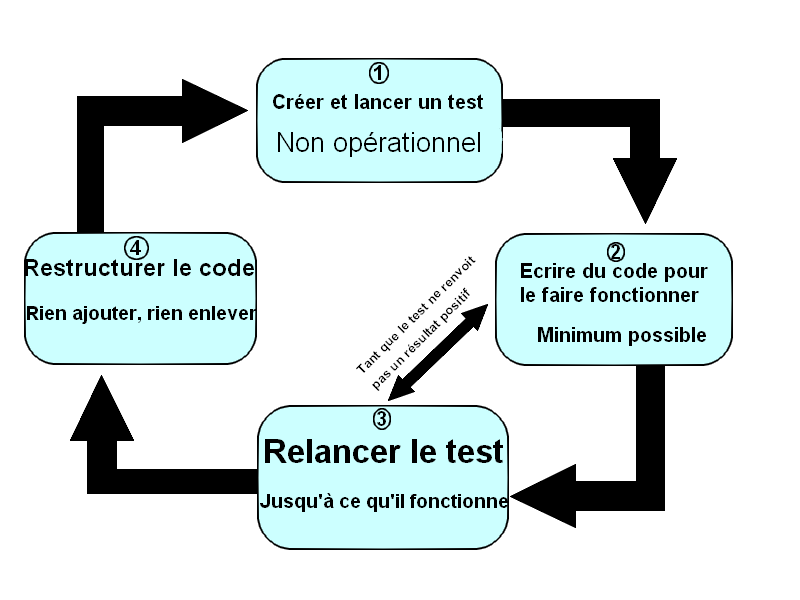
\includegraphics[width=0.500\linewidth]{TDD.png}
\caption{Schéma résumant les 4 étapes du Développement dirigé par les tests}\end{figure}


\section{Gain de temps?}
\label{tdd:gain-de-temps}
En lisant ces 4 étapes répétitives, on ne peut que se demander si le Test
Driven Development et son cycle compliqué est réellement un atout et un gain
de temps pour le programmeur.

Il est clair que, sur un travail de petite taille, tout coder n'aurait pas
énormément de sens, car tout peut être facilement essayable par soi-même.
Dans le cas d'un travail d'une certaine consistance, ce n'est pas pareil.
C'est uniquement en testant que l'on peut être sûr de son code, car cela
signifie qu'il est valide et devrait le rester.


\chapter{Débuter un projet}
\label{projet1:debuter-un-projet}\label{projet1::doc}
Pour comprendre grâce à la pratique, nous allons au cours de ce travail établir
un dashboard permettant à un professeur de gérer des classes et des exercices
sur un site d'e-learning pour les mathématiques grâce à Django, un framework
fonctionnant avec Python.


\section{Eléments requis}
\label{projet1:elements-requis}
Pour pouvoir parfaitement suivre ce guide, il nous faudra les éléments suivants
afin de réaliser les tests:
\begin{itemize}
\item {} 
\textbf{Django 1.7:} en effet, il va vous falloir django, car c'est le framework
que l'on va utiliser. Pour le télécharger, il suffit de taper la commande
suivante avec pip:

\begin{Verbatim}[commandchars=\\\{\}]
sudo pip3 install django==1.7
\end{Verbatim}

Si vous utilisez Windows, vous pouvez enlever \emph{sudo}.

\item {} 
\textbf{Selenium:} Selenium est un outil permettant de gérer les navigateurs
avec des commandes. Ceci nous sera utile pour les tests fonctionnels (ce
terme sera expliqué plus tard). Encore une fois, il est possible de le
télécharger grâce à pip:

\begin{Verbatim}[commandchars=\\\{\}]
sudo pip3 install \PYGZhy{}\PYGZhy{}upgrade selenium
\end{Verbatim}

Encore une fois, le \emph{sudo} n'est pas nécessaire sur Windows.

Note: il est important de toujours utiliser la dernière version de Selenium.
En effet, une version dépassée peut facilement se comporter de façon non
désirée. \footnote{
PERCIVAL, Harry J.W., «Test Driven Development With Python», publié
le 19 juin 2014
}

\end{itemize}

Une fois les éléments nécessaires installés, vous pouvez passer à la suite.


\section{Premier test}
\label{projet1:premier-test}
Le principe de base du Test Driven Development est d'écrire un test avant même
de coder ce que le test doit vérifier. Pour notre exemple, on devrait vérifier
qu'il y ait le plus basique des éléments sur notre site: Django. On va donc
créer un test fonctionnel pour voir s'il y a bien le titre de Django sur la page
d'accueil. Le test fonctionnel permet de nous assurer que notre site fonctionne
et possède la fonctionnalité la plus optimale qu'il soit.

Commençons donc par écrire ce code:

\begin{Verbatim}[commandchars=\\\{\},numbers=left,firstnumber=1,stepnumber=1]
\PYG{k+kn}{from} \PYG{n+nn}{selenium} \PYG{k+kn}{import} \PYG{n}{webdriver}

\PYG{n}{browser} \PYG{o}{=} \PYG{n}{webdriver}\PYG{o}{.}\PYG{n}{Firefox}\PYG{p}{(}\PYG{p}{)}
\PYG{n}{browser}\PYG{o}{.}\PYG{n}{get}\PYG{p}{(}\PYG{l+s}{\PYGZdq{}}\PYG{l+s}{http://localhost:8000}\PYG{l+s}{\PYGZdq{}}\PYG{p}{)}

\PYG{k}{assert} \PYG{l+s}{\PYGZdq{}}\PYG{l+s}{Django}\PYG{l+s}{\PYGZdq{}} \PYG{o+ow}{in} \PYG{n}{browser}\PYG{o}{.}\PYG{n}{title}

\PYG{n}{browser}\PYG{o}{.}\PYG{n}{quit}\PYG{p}{(}\PYG{p}{)}
\end{Verbatim}

Regardons une par une les lignes qui pourrait poser des problèmes de
compréhensions:
\begin{enumerate}
\item {} 
Nous permet d'importer webdriver qui nous sera utile pour gérer les
navigateurs web (dans ce cas, Firefox), nous permettant de les ouvrir,
d'aller à une URL ou de les fermer.

\end{enumerate}
\begin{enumerate}
\setcounter{enumi}{5}
\item {} 
Va basiquement nous dire si la page que l'on vient de charger
(\href{http://localhost:8000}{http://localhost:8000}) contient le mot ``Django'' dans le titre.

\end{enumerate}

Comme on peut s'y attendre, du moins si on se rappelle du but d'un test, le test
ne marchera pas. En effet, comme dit précédemment, les tests sont faits pour
évaluer quelque chose que l'on n'a pas encore fait, et pour nous aider à les
faire le plus simplement possible.

\textbf{Quand on test, il ne faut pas avoir les tests qui échouent comme quelque chose
de mal. Dans certains cas ( comme celui-ci), ces tests sont attendus et recevoir
un} \emph{False} \textbf{à la fin est donc un bon signe: notre test marche!}
\paragraph{Note de bas de page}



\renewcommand{\indexname}{Index}
\printindex
\end{document}
